% Options for packages loaded elsewhere
\PassOptionsToPackage{unicode}{hyperref}
\PassOptionsToPackage{hyphens}{url}
\PassOptionsToPackage{dvipsnames,svgnames,x11names}{xcolor}
%
\documentclass[
  authoryear,
  preprint,
  3p]{elsarticle}

\usepackage{amsmath,amssymb}
\usepackage{iftex}
\ifPDFTeX
  \usepackage[T1]{fontenc}
  \usepackage[utf8]{inputenc}
  \usepackage{textcomp} % provide euro and other symbols
\else % if luatex or xetex
  \usepackage{unicode-math}
  \defaultfontfeatures{Scale=MatchLowercase}
  \defaultfontfeatures[\rmfamily]{Ligatures=TeX,Scale=1}
\fi
\usepackage{lmodern}
\ifPDFTeX\else  
    % xetex/luatex font selection
\fi
% Use upquote if available, for straight quotes in verbatim environments
\IfFileExists{upquote.sty}{\usepackage{upquote}}{}
\IfFileExists{microtype.sty}{% use microtype if available
  \usepackage[]{microtype}
  \UseMicrotypeSet[protrusion]{basicmath} % disable protrusion for tt fonts
}{}
\makeatletter
\@ifundefined{KOMAClassName}{% if non-KOMA class
  \IfFileExists{parskip.sty}{%
    \usepackage{parskip}
  }{% else
    \setlength{\parindent}{0pt}
    \setlength{\parskip}{6pt plus 2pt minus 1pt}}
}{% if KOMA class
  \KOMAoptions{parskip=half}}
\makeatother
\usepackage{xcolor}
\setlength{\emergencystretch}{3em} % prevent overfull lines
\setcounter{secnumdepth}{5}
% Make \paragraph and \subparagraph free-standing
\ifx\paragraph\undefined\else
  \let\oldparagraph\paragraph
  \renewcommand{\paragraph}[1]{\oldparagraph{#1}\mbox{}}
\fi
\ifx\subparagraph\undefined\else
  \let\oldsubparagraph\subparagraph
  \renewcommand{\subparagraph}[1]{\oldsubparagraph{#1}\mbox{}}
\fi


\providecommand{\tightlist}{%
  \setlength{\itemsep}{0pt}\setlength{\parskip}{0pt}}\usepackage{longtable,booktabs,array}
\usepackage{calc} % for calculating minipage widths
% Correct order of tables after \paragraph or \subparagraph
\usepackage{etoolbox}
\makeatletter
\patchcmd\longtable{\par}{\if@noskipsec\mbox{}\fi\par}{}{}
\makeatother
% Allow footnotes in longtable head/foot
\IfFileExists{footnotehyper.sty}{\usepackage{footnotehyper}}{\usepackage{footnote}}
\makesavenoteenv{longtable}
\usepackage{graphicx}
\makeatletter
\def\maxwidth{\ifdim\Gin@nat@width>\linewidth\linewidth\else\Gin@nat@width\fi}
\def\maxheight{\ifdim\Gin@nat@height>\textheight\textheight\else\Gin@nat@height\fi}
\makeatother
% Scale images if necessary, so that they will not overflow the page
% margins by default, and it is still possible to overwrite the defaults
% using explicit options in \includegraphics[width, height, ...]{}
\setkeys{Gin}{width=\maxwidth,height=\maxheight,keepaspectratio}
% Set default figure placement to htbp
\makeatletter
\def\fps@figure{htbp}
\makeatother

\usepackage{fontspec}
\usepackage{multirow}
\usepackage{multicol}
\usepackage{colortbl}
\usepackage{hhline}
\newlength\Oldarrayrulewidth
\newlength\Oldtabcolsep
\usepackage{longtable}
\usepackage{array}
\usepackage{hyperref}
\usepackage{float}
\usepackage{wrapfig}
\usepackage{graphicx}
\usepackage{unicode-math}
\usepackage{hyperref}
\def\tightlist{}
\usepackage{setspace}
\doublespacing
\usepackage{lineno}
\linenumbers
\makeatletter
\makeatother
\makeatletter
\makeatother
\makeatletter
\@ifpackageloaded{caption}{}{\usepackage{caption}}
\AtBeginDocument{%
\ifdefined\contentsname
  \renewcommand*\contentsname{Table of contents}
\else
  \newcommand\contentsname{Table of contents}
\fi
\ifdefined\listfigurename
  \renewcommand*\listfigurename{List of Figures}
\else
  \newcommand\listfigurename{List of Figures}
\fi
\ifdefined\listtablename
  \renewcommand*\listtablename{List of Tables}
\else
  \newcommand\listtablename{List of Tables}
\fi
\ifdefined\figurename
  \renewcommand*\figurename{Figure}
\else
  \newcommand\figurename{Figure}
\fi
\ifdefined\tablename
  \renewcommand*\tablename{Table}
\else
  \newcommand\tablename{Table}
\fi
}
\@ifpackageloaded{float}{}{\usepackage{float}}
\floatstyle{ruled}
\@ifundefined{c@chapter}{\newfloat{codelisting}{h}{lop}}{\newfloat{codelisting}{h}{lop}[chapter]}
\floatname{codelisting}{Listing}
\newcommand*\listoflistings{\listof{codelisting}{List of Listings}}
\makeatother
\makeatletter
\@ifpackageloaded{caption}{}{\usepackage{caption}}
\@ifpackageloaded{subcaption}{}{\usepackage{subcaption}}
\makeatother
\makeatletter
\@ifpackageloaded{tcolorbox}{}{\usepackage[skins,breakable]{tcolorbox}}
\makeatother
\makeatletter
\@ifundefined{shadecolor}{\definecolor{shadecolor}{rgb}{.97, .97, .97}}
\makeatother
\makeatletter
\makeatother
\makeatletter
\makeatother
\journal{Journal of Transport Geography}
\ifLuaTeX
  \usepackage{selnolig}  % disable illegal ligatures
\fi
\usepackage[]{natbib}
\bibliographystyle{elsarticle-harv}
\IfFileExists{bookmark.sty}{\usepackage{bookmark}}{\usepackage{hyperref}}
\IfFileExists{xurl.sty}{\usepackage{xurl}}{} % add URL line breaks if available
\urlstyle{same} % disable monospaced font for URLs
\hypersetup{
  pdftitle={Exploring mobility of care with measures of access: a case for gender-mainstreaming accessibility analysis},
  pdfauthor={AAA; BBB; CCC},
  pdfkeywords={Accessibility, Mobility of Care, Gender, Cumulative
Opportunity, Spatial Availability},
  colorlinks=true,
  linkcolor={blue},
  filecolor={Maroon},
  citecolor={Blue},
  urlcolor={Blue},
  pdfcreator={LaTeX via pandoc}}

\setlength{\parindent}{6pt}
\begin{document}

\begin{frontmatter}
\title{Exploring mobility of care with measures of access: a case for
gender-mainstreaming accessibility analysis}
\author[]{AAA%
\corref{cor1}%
}
 \ead{AAA@AAA} 
\author[]{BBB%
%
}
 \ead{BBB@BBB} 
\author[]{CCC%
%
}
 \ead{CCC@CCC} 


\cortext[cor1]{Corresponding author}



        
\begin{abstract}
Accessibility, the ease of interacting with opportunities, is an
increasingly important tool amongst transport planners aiming to foster
equitable and sustainable cities. However, in accessibility research
there is a masculinist bias whereby employment destinations are often
the default. This paper aims to counter this gendered bias by connecting
the Mobility of Care conceptualisation to an empirical accessibility
analysis of care destinations in the City of Hamilton, Canada. Care
destinations are all the places one must visit to sustain household
needs such shopping, errands, and caring for others (children and other
dependents). Through the creation of a novel care destination dataset,
this paper considers access to care across different modes of transport
at two travel time thresholds (trips shorter than 15-minutes and
30-minutes) using unconstrained (cumulative opportunity) and
competitive-constrained (spatial availability) measures. Results
generally indicate that travel to care destinations by car is
exceptionally high, and access by public transit, cycling and by foot is
low across the city with some exceptions in the inner city. Noteably,
there are distinctions between both methods: unconstrained access
illustrates a more optimistic landscape for non-car modes, while
competitive and constrained access demonstrates a conceptually more
realistic spatial distribution of care destination availability.
Neighbourhoods with both low spatial availability to care and a high
proportion of low-income households are also identified as areas in need
of intervention. The manuscript and analysis is computationally
reproducible and openly available. The analysis presented demonstrates
methods planners can use to gender-mainstream accessibility analysis.
Further, results can inform policies aiming to encourage sustainable
mobility.
\end{abstract}





\begin{keyword}
    Accessibility \sep Mobility of Care \sep Gender \sep Cumulative
Opportunity \sep 
    Spatial Availability
\end{keyword}
\end{frontmatter}
    \ifdefined\Shaded\renewenvironment{Shaded}{\begin{tcolorbox}[enhanced, interior hidden, breakable, borderline west={3pt}{0pt}{shadecolor}, boxrule=0pt, frame hidden, sharp corners]}{\end{tcolorbox}}\fi

\hypertarget{introduction}{%
\section{Introduction}\label{introduction}}

A gender bias exists in transport research and policy
\citep{sanchezdemadariagaMobilityCareIntroducing2013, lawWomenTransportNew1999, siemiatyckiGenderedProductionInfrastructure2020}.
The field has historically focused on one trip purpose; the on-peak
commute to work. While many women do, of course, work, the commute is
still a travel pattern more frequent amongst men
\citep{sanchezdemadariagaMobilityCareIntroducing2013}. Women, on the
other hand, have been found to complete more household-serving travel
than men, such as escorting children
\citep{craigGenderMobilityParental2019, taylorWhatExplainsGender2015, hanTaskAllocationGender2019, mcdonaldExploratoryAnalysisChildren2006},
shopping, and errand trips
\citep{taylorWhatExplainsGender2015, rootWomenTravelIdea2000, sweetGenderDifferencesRole2016}.

Though research on the gendered distribution of household-serving travel
has existed for decades, it was only in 2013 that Sánchez de Madariaga
coined the term Mobility of Care, i.e., all the travel needed to fulfill
household needs (e.g., a combination of travel to grocery stores,
errands, and pick-up / drop-off of children)
\citep{sanchezdemadariagaMobilityCareIntroducing2013}. The term was
developed to highlight how these household-serving trips are
systematically under-represented, under-counted, and rendered invisible
due to masculinist biases in transport planning. Take, for instance, how
trips to household sustaining destinations are categorized in typical
large-scale travel surveys
\citep{sanchezdemadariagaMobilityCareIntroducing2013}. In the Greater
Golden Horseshoe Area's (encompassing the Greater Toronto and Hamilton
Area) Transportation Tomorrow Survey (TTS)
\citep{transportationtomorrowsurvey2018} respondents are given the
following options to categorize their trip origins and destinations:
home, work, school, daycare, facilitate passenger, marketing/shopping,
other, or unknown. While home-work and home-school trips are easily
identified, care trips are more challenging to measure. Many
marketing/shopping trips are likely for care purposes (e.g., groceries),
but others are likely for leisure. While escort trips are likely well
captured under the categories `daycare' or `facilitate passenger', trips
to run errands or to attend health appointments are not clearly
captured. It is probable that responds categorize many of these trips as
`other' or even `unknown'. The focus of the survey is on what is a
`typical' trip to work or school
\citep{transportationtomorrowsurvey2018}; other trips are a by-product,
`non-typical' and minimialised in importance. Of course, people's travel
behaviours are complex and surveys must balance detail with summary.
However, what is seen as a `typical' trip continues to shape transport
and land-use, and this aggregation steers data-driven solutions from
counted and observed home -work/-school based trips.

When travel surveys are designed to explicitly capture mobility of care,
preliminary research has found that it comprises approximately one third
of adults' trips
\citep{gomezvaroAccountingCareEveryday2023, sanchezdemadariagaMobilityCareIntroducing2013, sanchezdemadariagaMeasuringMobilitiesCare2019, ravensbergenExploratoryAnalysisMobility2022}.
Given the large proportion of daily travel that mobility of care
comprises, these trips should be explicitly captured in transport
research. Further, the current under-reporting of mobility of care in
research and planning has important equity considerations. Not only are
mobility of care trips completed predominantly by women, this gendered
discrepancy is greater in low-income households
\citep{murillomunarCaregiversMoveGender2023, sanchezdemadariagaMobilityCareIntroducing2013, ravensbergenExploratoryAnalysisMobility2022}.
For instance, in lower income households in Montréal, women complete
50\% more care trips than men
\citep{ravensbergenExploratoryAnalysisMobility2022}.

The power of the Mobility of Care concept lies in its ability to
highlight the masculinist bias in transport research -- travel for care
appears insignificant because travel surveys are not written to capture
it \citep{sanchezdemadariagaMobilityCareIntroducing2013}. Travel
surveys, however, are but one tool used by transport researchers and
practitioners. Another popular tool in transport planning and research
is accessibility, an indicator that quantifies ``the potential of
opportunities for interaction'' as defined in the seminal work of Hansen
\citep{hansenHowAccessibilityShapes1959}. Accessibility indicators can
be interpreted as the ease of reaching destinations using transport
networks: a byproduct of mobility and a representation of the people's
interaction with land-use and transportation systems
\citep{hansenHowAccessibilityShapes1959, handyAccessibilityIdeaWhose2020, elgeneidyMakingAccessibilityWork2021}.
The points of interest in many accessibility-based assessments have been
home-to-work destinations
\citep{kelobonyeRelativeAccessibilityAnalysis2019, farberOntarioLineSocioeconomic2019, duarteInfluenceJobAccessibility2023, ryanAccessibilitySpaceTime2023}.
For example, in the accessibility assessment of the Ontario Line, a
subway line that will be constructed in the city of Toronto, Canada,
Farber and Allen \citep{farberOntarioLineSocioeconomic2019} highlight
how this new investment will increase access to jobs for residents
across the City by 1.14\% overall. While much has been learned, shifting
focus from jobs as the default destination may open opportunities for
gender-mainstreaming accessibility analyses. Indeed, jobs are not always
the most significant destination for many segments of the population. As
discussed, women's commutes comprise on average a smaller proportion of
their daily travel than men's
\citep{ravensbergenExploratoryAnalysisMobility2022}. This focus on
job-access can additionally bias accessibility-gains that children and
older adults who reside in impacted areas may see as well
\citep{grantsmithManagingChallengesCombining2016}. One way to counter
this bias is to reframe accessibility analysis by explicitly considering
destinations involved in mobility of care.

Reframing accessibility analyses to incorporate mobility of care is also
pertinent to the promotion of sustainable travel modes in cities.
Research has found that people are less likely to use public transport
or bicycles for care trips
\citep{ravensbergenExploratoryAnalysisMobility2022} and more likely to
make these trips by car
\citep{maciejewskaHaveChildrenThus2019, ravensbergenExploratoryAnalysisMobility2022}.
A lack of access to care destinations by bicycle and transit may
contribute to these trends. Mobility of care is also more commonly
completed by foot than the commute to work
\citep{ravensbergenExploratoryAnalysisMobility2022}. Whether there is a
relationship between these travel behaviors and people's access to care
destination using different modes, however, remains unknown, as mobility
of care is largely uncounted in transport research.

In this spirit, this study foregrounds the theoretical mobility of care
concept by calculating the accessibility to care destinations or
multiple modes in an empirical case study of Hamilton, Canada. Two
place-based accessibility measures are used to motivate the discussion:
one unconstrained measure (cumulative opportunity) and another
competitive and constrained measure (spatial availability
\citep{soukhovIntroducingSpatialAvailability2023}). The cumulative
opportunity measure demonstrates the potential access to all
destinations within 15-minutes and 30-minutes. This measure is widely
appreciated for its intuitive computation
\citep{handyAccessibilityIdeaWhose2020, handyMeasuringAccessibilityExploration1997, kelobonyeRelativeAccessibilityAnalysis2019, chengInvestigatingWalkingAccessibility2019}
but critiqued for its omission of competition effects
\citep{paezDemand2019, soukhovIntroducingSpatialAvailability2023, kelobonyeMeasuringAccessibilitySpatial2020, merlinDoesCompetitionMatter2017}.
To respond to this critic, spatial availability of care destinations per
mode is also calculated as an additional and arguably more conceptually
realistic reflection of opportunity availability. This research aims to
contribute to gender-mainstreaming in transport planning by
demonstrating an approach to a feminist accessibility calculation
through these two accessibility measures.

\hypertarget{background-and-methods}{%
\section{Background and methods}\label{background-and-methods}}

This paper focuses on Hamilton, a mid-size city of approximately 500,000
residents that lies within the urban and suburban Greater Toronto and
Hamilton Area (GTHA) \citep{transportationtomorrowsurvey2018}. The GTHA
is home to seven million people, or approximately 20\% of the Canadian
population \citep{cityoftoronto2021CensusPopulationa2022}. Hamilton is
divided into six regional communities (Figure~\ref{fig-Fig1}).
Hamilton-Central is the densest and most urbanized of the six, and the
five periphery communities of Dundas, Ancaster, Flamborough, Glanbrook
and Stoney Creek are significantly more suburbanized with the furthest
periphery regions being undeveloped or rural owing to their inclusion in
the region's greenbelt
\citep{greenbeltfoundationThrivingGreenbeltThriving2023}. These
different urban forms and associated transport infrastructure play a key
role in access to care destinations.

Further, the entire manuscript and all analysis is conducted in R and
RStudio. All work is computationally reproducible and openly available
in the lead author's \href{XXX}{GitHub repository}.

\begin{figure}

{\centering 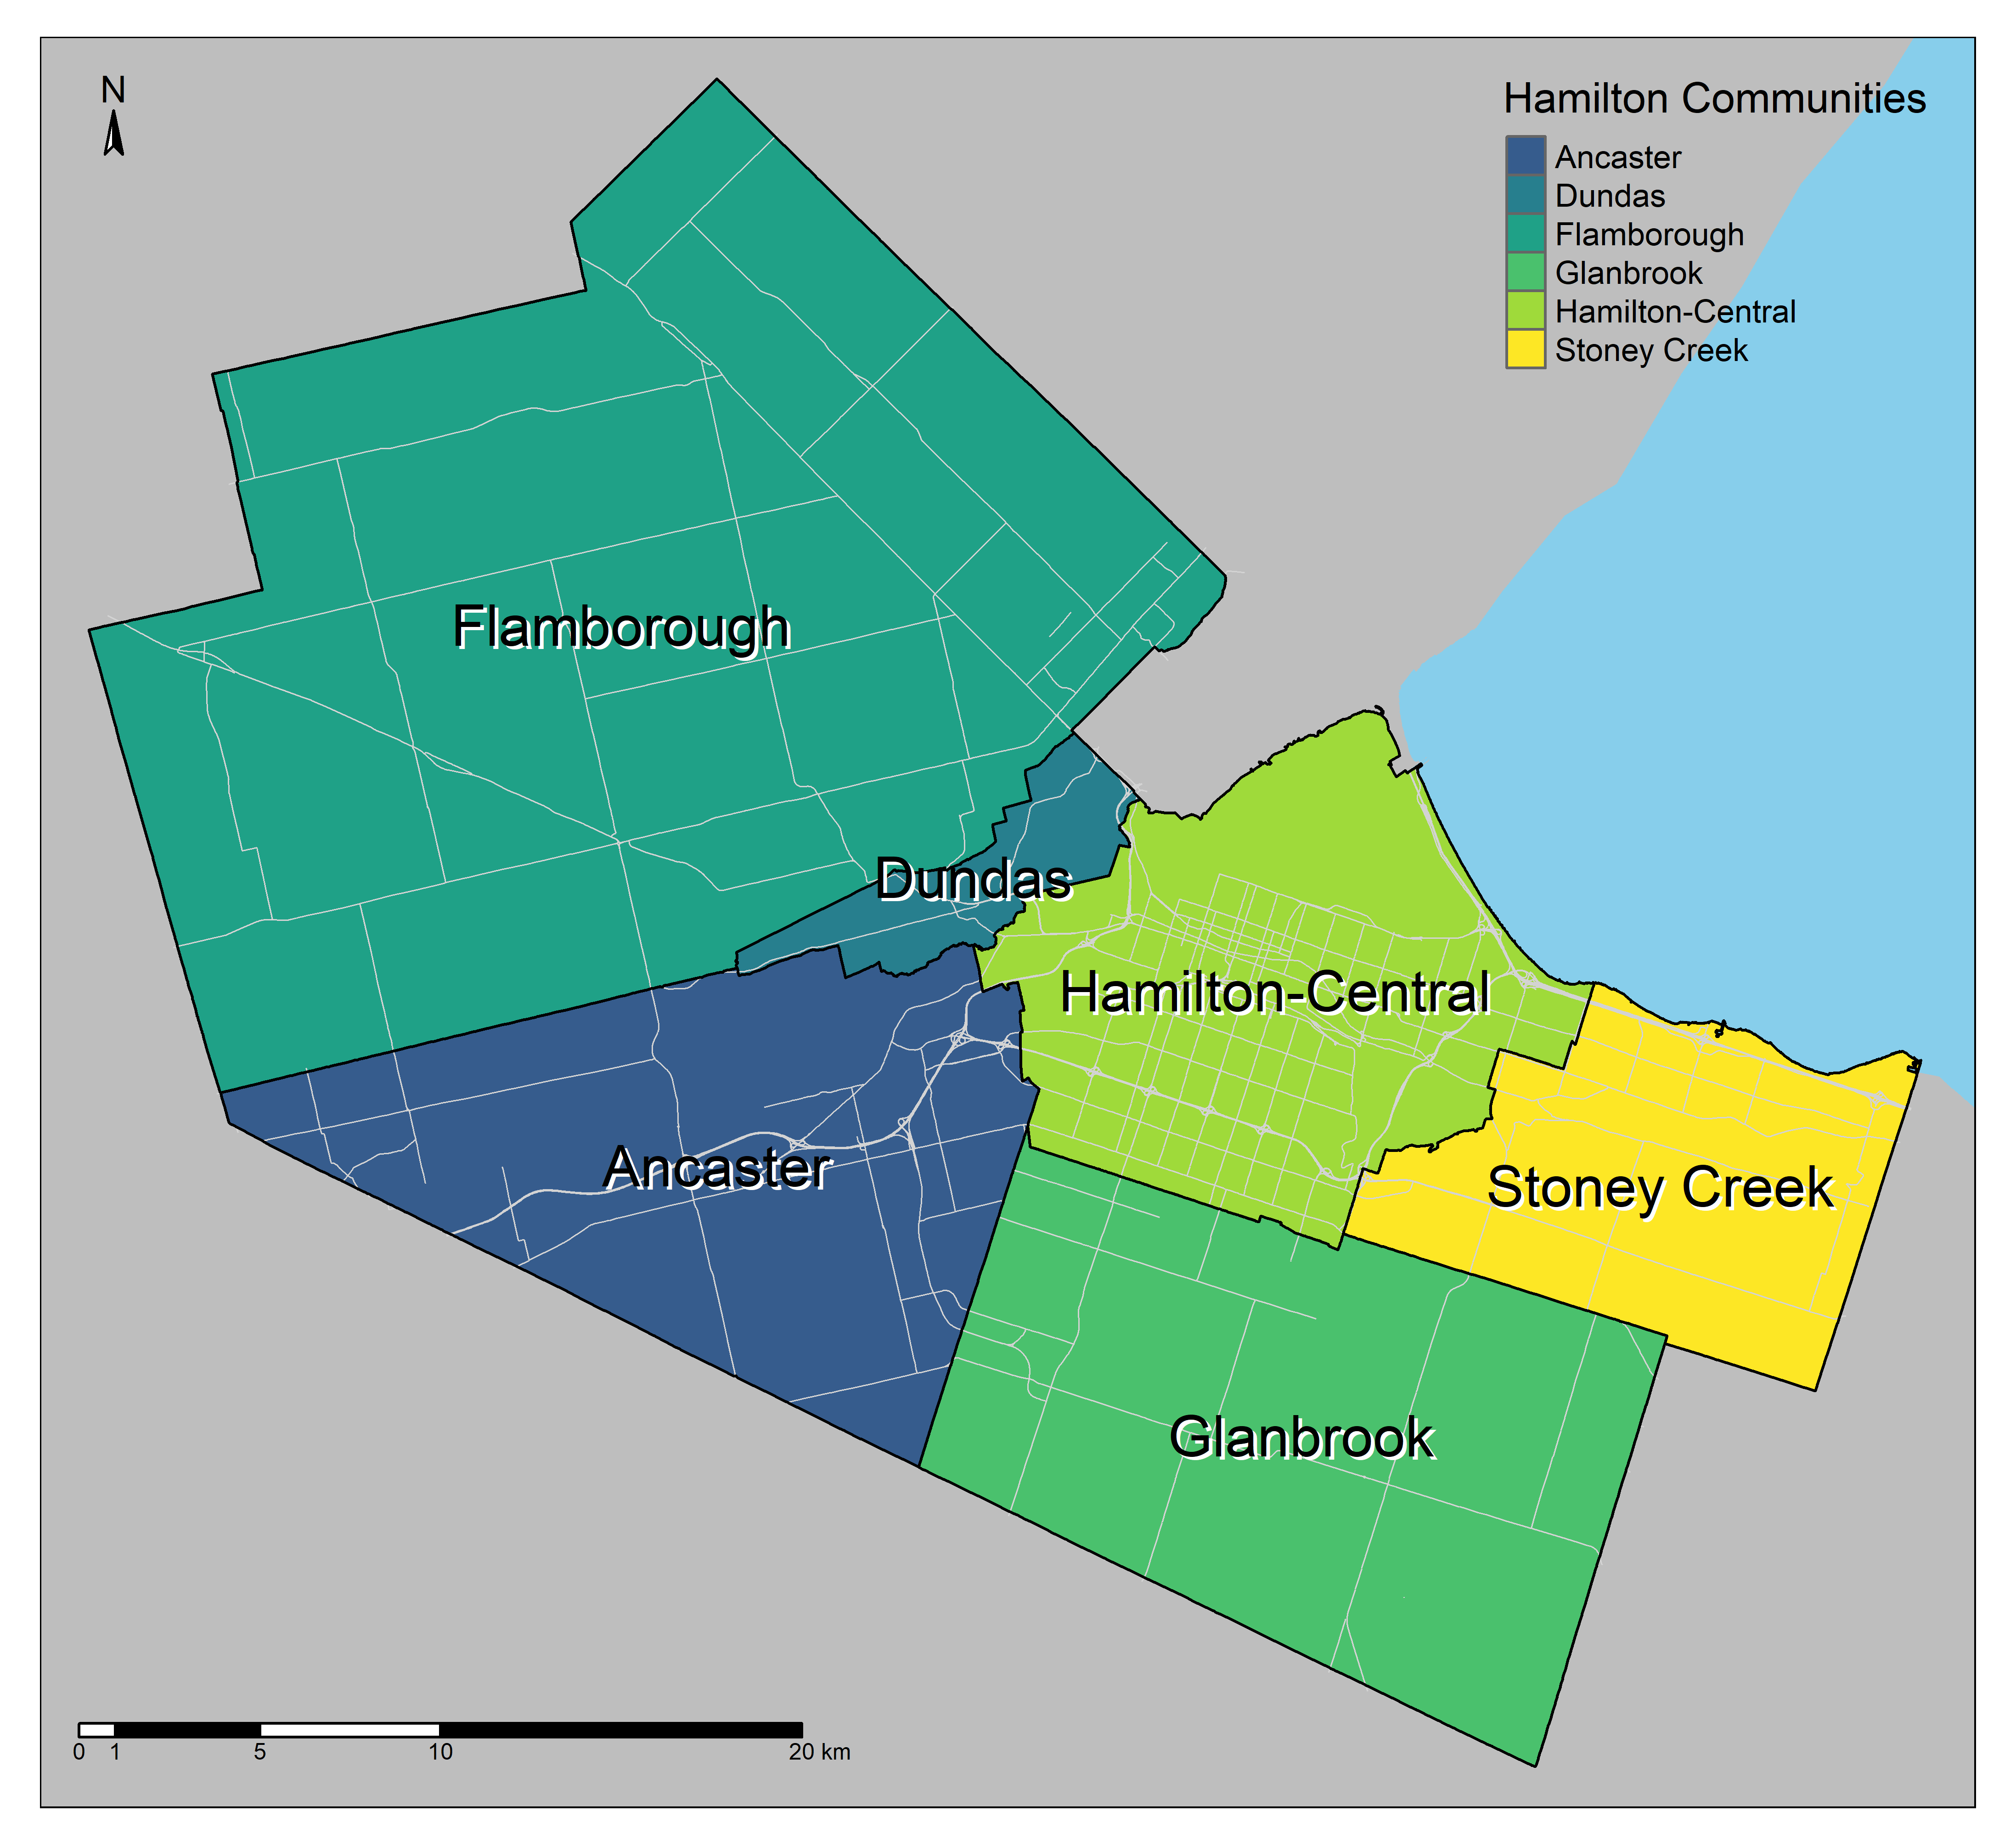
\includegraphics[width=6.25in,height=\textheight]{figures/Fig1-boundaries.png}

}

\caption{\label{fig-Fig1}The six former muncipal boundaries in the city
of Hamilton. Basemap shapefiles are retrieved from the Open Data
Hamilton Portal \citep{opendatahamiltonCityBoundary2023} and the USGS
\citep{greatlakesUSGS2010}. Highways and arterial roads are shown in
light grey.}

\end{figure}

\hypertarget{destination-dataset}{%
\subsection{Destination dataset}\label{destination-dataset}}

A geospatial dataset of care destinations for Hamilton (e.g., full
addresses of longitude and latitude) was compiled. The geospatial data
was sourced from provincial and municipal open data portals
\citep{governmentofontarioOntarioDataCatalogue2023, cityofhamiltonOpenData2023},
Data Axle, a consumer dataset compiled of businesses and companies
within Canada \citep{axledataConsumerData2023} or manually through
Google Maps. Each destination was categorized based on the specific type
of care being accessed following the mobility of care research by
Sanchez de Madariaga \& Zucchini (2019)
\citep{sanchezdemadariagaMeasuringMobilitiesCare2019}. Categories
include child, elder, grocery, health, and errand -centric destinations.
Category sources of data and preparation notes are detailed in
Table~\ref{tbl-Tbl1}. Their spatial distribution and sub-categories are
visualised in Figure~\ref{fig-Fig2}.

\hypertarget{tbl-Tbl1}{}
\global\setlength{\Oldarrayrulewidth}{\arrayrulewidth}

\global\setlength{\Oldtabcolsep}{\tabcolsep}

\setlength{\tabcolsep}{0pt}

\renewcommand*{\arraystretch}{1.5}



\providecommand{\ascline}[3]{\noalign{\global\arrayrulewidth #1}\arrayrulecolor[HTML]{#2}\cline{#3}}

\begin{longtable}[c]{|p{0.67in}|p{1.69in}|p{4.33in}}
\caption{\label{tbl-Tbl1}Details on the preparation and data sources of care destinations. }\tabularnewline




\ascline{1.5pt}{666666}{1-3}

\multicolumn{1}{>{\raggedright}m{\dimexpr 0.67in+0\tabcolsep}}{\textcolor[HTML]{000000}{\fontsize{10}{10}\selectfont{Care\ category}}} & \multicolumn{1}{>{\raggedright}m{\dimexpr 1.69in+0\tabcolsep}}{\textcolor[HTML]{000000}{\fontsize{10}{10}\selectfont{Sources}}} & \multicolumn{1}{>{\raggedright}m{\dimexpr 4.33in+0\tabcolsep}}{\textcolor[HTML]{000000}{\fontsize{10}{10}\selectfont{Data\ preparation\ notes}}} \\

\ascline{1.5pt}{666666}{1-3}\endfirsthead 

\ascline{1.5pt}{666666}{1-3}

\multicolumn{1}{>{\raggedright}m{\dimexpr 0.67in+0\tabcolsep}}{\textcolor[HTML]{000000}{\fontsize{10}{10}\selectfont{Care\ category}}} & \multicolumn{1}{>{\raggedright}m{\dimexpr 1.69in+0\tabcolsep}}{\textcolor[HTML]{000000}{\fontsize{10}{10}\selectfont{Sources}}} & \multicolumn{1}{>{\raggedright}m{\dimexpr 4.33in+0\tabcolsep}}{\textcolor[HTML]{000000}{\fontsize{10}{10}\selectfont{Data\ preparation\ notes}}} \\

\ascline{1.5pt}{666666}{1-3}\endhead



\multicolumn{1}{>{\raggedright}m{\dimexpr 0.67in+0\tabcolsep}}{\textcolor[HTML]{000000}{\fontsize{10}{10}\selectfont{Child-centric}}} & \multicolumn{1}{>{\raggedright}m{\dimexpr 1.69in+0\tabcolsep}}{\textcolor[HTML]{000000}{\fontsize{10}{10}\selectfont{(Hamilton}}\textcolor[HTML]{000000}{\fontsize{10}{10}\selectfont{\ }}\textcolor[HTML]{000000}{\fontsize{10}{10}\selectfont{2022a,}}\textcolor[HTML]{000000}{\fontsize{10}{10}\selectfont{\ }}\textcolor[HTML]{000000}{\fontsize{10}{10}\selectfont{2023,}}\textcolor[HTML]{000000}{\fontsize{10}{10}\selectfont{\ }}\textcolor[HTML]{000000}{\fontsize{10}{10}\selectfont{2022c,}}\textcolor[HTML]{000000}{\fontsize{10}{10}\selectfont{\ }}\textcolor[HTML]{000000}{\fontsize{10}{10}\selectfont{2022d;}}\textcolor[HTML]{000000}{\fontsize{10}{10}\selectfont{\ }}\textcolor[HTML]{000000}{\fontsize{10}{10}\selectfont{Ontario}}\textcolor[HTML]{000000}{\fontsize{10}{10}\selectfont{\ }}\textcolor[HTML]{000000}{\fontsize{10}{10}\selectfont{2023b)}}} & \multicolumn{1}{>{\raggedright}m{\dimexpr 4.33in+0\tabcolsep}}{\textcolor[HTML]{000000}{\fontsize{10}{10}\selectfont{Schools,}}\textcolor[HTML]{000000}{\fontsize{10}{10}\selectfont{\ }}\textcolor[HTML]{000000}{\fontsize{10}{10}\selectfont{daycares,}}\textcolor[HTML]{000000}{\fontsize{10}{10}\selectfont{\ }}\textcolor[HTML]{000000}{\fontsize{10}{10}\selectfont{and}}\textcolor[HTML]{000000}{\fontsize{10}{10}\selectfont{\ }}\textcolor[HTML]{000000}{\fontsize{10}{10}\selectfont{community}}\textcolor[HTML]{000000}{\fontsize{10}{10}\selectfont{\ }}\textcolor[HTML]{000000}{\fontsize{10}{10}\selectfont{centres,}}\textcolor[HTML]{000000}{\fontsize{10}{10}\selectfont{\ }}\textcolor[HTML]{000000}{\fontsize{10}{10}\selectfont{recreation}}\textcolor[HTML]{000000}{\fontsize{10}{10}\selectfont{\ }}\textcolor[HTML]{000000}{\fontsize{10}{10}\selectfont{centres,}}\textcolor[HTML]{000000}{\fontsize{10}{10}\selectfont{\ }}\textcolor[HTML]{000000}{\fontsize{10}{10}\selectfont{and}}\textcolor[HTML]{000000}{\fontsize{10}{10}\selectfont{\ }}\textcolor[HTML]{000000}{\fontsize{10}{10}\selectfont{parks:}}\textcolor[HTML]{000000}{\fontsize{10}{10}\selectfont{\ }}\textcolor[HTML]{000000}{\fontsize{10}{10}\selectfont{1,190}}\textcolor[HTML]{000000}{\fontsize{10}{10}\selectfont{\ }}\textcolor[HTML]{000000}{\fontsize{10}{10}\selectfont{locations}}\textcolor[HTML]{000000}{\fontsize{10}{10}\selectfont{\ }}\textcolor[HTML]{000000}{\fontsize{10}{10}\selectfont{are}}\textcolor[HTML]{000000}{\fontsize{10}{10}\selectfont{\ }}\textcolor[HTML]{000000}{\fontsize{10}{10}\selectfont{included.}}\textcolor[HTML]{000000}{\fontsize{10}{10}\selectfont{\ }}\textcolor[HTML]{000000}{\fontsize{10}{10}\selectfont{After}}\textcolor[HTML]{000000}{\fontsize{10}{10}\selectfont{\ }}\textcolor[HTML]{000000}{\fontsize{10}{10}\selectfont{manual}}\textcolor[HTML]{000000}{\fontsize{10}{10}\selectfont{\ }}\textcolor[HTML]{000000}{\fontsize{10}{10}\selectfont{review,}}\textcolor[HTML]{000000}{\fontsize{10}{10}\selectfont{\ }}\textcolor[HTML]{000000}{\fontsize{10}{10}\selectfont{all}}\textcolor[HTML]{000000}{\fontsize{10}{10}\selectfont{\ }}\textcolor[HTML]{000000}{\fontsize{10}{10}\selectfont{locations}}\textcolor[HTML]{000000}{\fontsize{10}{10}\selectfont{\ }}\textcolor[HTML]{000000}{\fontsize{10}{10}\selectfont{that}}\textcolor[HTML]{000000}{\fontsize{10}{10}\selectfont{\ }}\textcolor[HTML]{000000}{\fontsize{10}{10}\selectfont{typically}}\textcolor[HTML]{000000}{\fontsize{10}{10}\selectfont{\ }}\textcolor[HTML]{000000}{\fontsize{10}{10}\selectfont{do}}\textcolor[HTML]{000000}{\fontsize{10}{10}\selectfont{\ }}\textcolor[HTML]{000000}{\fontsize{10}{10}\selectfont{not}}\textcolor[HTML]{000000}{\fontsize{10}{10}\selectfont{\ }}\textcolor[HTML]{000000}{\fontsize{10}{10}\selectfont{serve}}\textcolor[HTML]{000000}{\fontsize{10}{10}\selectfont{\ }}\textcolor[HTML]{000000}{\fontsize{10}{10}\selectfont{children}}\textcolor[HTML]{000000}{\fontsize{10}{10}\selectfont{\ }}\textcolor[HTML]{000000}{\fontsize{10}{10}\selectfont{were}}\textcolor[HTML]{000000}{\fontsize{10}{10}\selectfont{\ }}\textcolor[HTML]{000000}{\fontsize{10}{10}\selectfont{removed}}\textcolor[HTML]{000000}{\fontsize{10}{10}\selectfont{\ }}\textcolor[HTML]{000000}{\fontsize{10}{10}\selectfont{including:}}\textcolor[HTML]{000000}{\fontsize{10}{10}\selectfont{\ }}\textcolor[HTML]{000000}{\fontsize{10}{10}\selectfont{Post-Secondary,}}\textcolor[HTML]{000000}{\fontsize{10}{10}\selectfont{\ }}\textcolor[HTML]{000000}{\fontsize{10}{10}\selectfont{Adult-Learning}}\textcolor[HTML]{000000}{\fontsize{10}{10}\selectfont{\ }}\textcolor[HTML]{000000}{\fontsize{10}{10}\selectfont{Centres,}}\textcolor[HTML]{000000}{\fontsize{10}{10}\selectfont{\ }}\textcolor[HTML]{000000}{\fontsize{10}{10}\selectfont{Group}}\textcolor[HTML]{000000}{\fontsize{10}{10}\selectfont{\ }}\textcolor[HTML]{000000}{\fontsize{10}{10}\selectfont{Homes,}}\textcolor[HTML]{000000}{\fontsize{10}{10}\selectfont{\ }}\textcolor[HTML]{000000}{\fontsize{10}{10}\selectfont{and}}\textcolor[HTML]{000000}{\fontsize{10}{10}\selectfont{\ }}\textcolor[HTML]{000000}{\fontsize{10}{10}\selectfont{Foster}}\textcolor[HTML]{000000}{\fontsize{10}{10}\selectfont{\ }}\textcolor[HTML]{000000}{\fontsize{10}{10}\selectfont{Care}}\textcolor[HTML]{000000}{\fontsize{10}{10}\selectfont{\ }}\textcolor[HTML]{000000}{\fontsize{10}{10}\selectfont{Centres.}}\textcolor[HTML]{000000}{\fontsize{10}{10}\selectfont{\ }}\textcolor[HTML]{000000}{\fontsize{10}{10}\selectfont{Further,}}\textcolor[HTML]{000000}{\fontsize{10}{10}\selectfont{\ }}\textcolor[HTML]{000000}{\fontsize{10}{10}\selectfont{through}}\textcolor[HTML]{000000}{\fontsize{10}{10}\selectfont{\ }}\textcolor[HTML]{000000}{\fontsize{10}{10}\selectfont{examination}}\textcolor[HTML]{000000}{\fontsize{10}{10}\selectfont{\ }}\textcolor[HTML]{000000}{\fontsize{10}{10}\selectfont{some}}\textcolor[HTML]{000000}{\fontsize{10}{10}\selectfont{\ }}\textcolor[HTML]{000000}{\fontsize{10}{10}\selectfont{Section}}\textcolor[HTML]{000000}{\fontsize{10}{10}\selectfont{\ }}\textcolor[HTML]{000000}{\fontsize{10}{10}\selectfont{23}}\textcolor[HTML]{000000}{\fontsize{10}{10}\selectfont{\ }}\textcolor[HTML]{000000}{\fontsize{10}{10}\selectfont{institutions}}\textcolor[HTML]{000000}{\fontsize{10}{10}\selectfont{\ }}\textcolor[HTML]{000000}{\fontsize{10}{10}\selectfont{defined}}\textcolor[HTML]{000000}{\fontsize{10}{10}\selectfont{\ }}\textcolor[HTML]{000000}{\fontsize{10}{10}\selectfont{as}}\textcolor[HTML]{000000}{\fontsize{10}{10}\selectfont{\ }}\textcolor[HTML]{000000}{\fontsize{10}{10}\selectfont{\textit{“}}}\textcolor[HTML]{000000}{\fontsize{10}{10}\selectfont{\textit{centres}}}\textcolor[HTML]{000000}{\fontsize{10}{10}\selectfont{\textit{\ }}}\textcolor[HTML]{000000}{\fontsize{10}{10}\selectfont{\textit{for}}}\textcolor[HTML]{000000}{\fontsize{10}{10}\selectfont{\textit{\ }}}\textcolor[HTML]{000000}{\fontsize{10}{10}\selectfont{\textit{children}}}\textcolor[HTML]{000000}{\fontsize{10}{10}\selectfont{\textit{\ }}}\textcolor[HTML]{000000}{\fontsize{10}{10}\selectfont{\textit{who}}}\textcolor[HTML]{000000}{\fontsize{10}{10}\selectfont{\textit{\ }}}\textcolor[HTML]{000000}{\fontsize{10}{10}\selectfont{\textit{cannot}}}\textcolor[HTML]{000000}{\fontsize{10}{10}\selectfont{\textit{\ }}}\textcolor[HTML]{000000}{\fontsize{10}{10}\selectfont{\textit{attend}}}\textcolor[HTML]{000000}{\fontsize{10}{10}\selectfont{\textit{\ }}}\textcolor[HTML]{000000}{\fontsize{10}{10}\selectfont{\textit{school}}}\textcolor[HTML]{000000}{\fontsize{10}{10}\selectfont{\textit{\ }}}\textcolor[HTML]{000000}{\fontsize{10}{10}\selectfont{\textit{to}}}\textcolor[HTML]{000000}{\fontsize{10}{10}\selectfont{\textit{\ }}}\textcolor[HTML]{000000}{\fontsize{10}{10}\selectfont{\textit{meet}}}\textcolor[HTML]{000000}{\fontsize{10}{10}\selectfont{\textit{\ }}}\textcolor[HTML]{000000}{\fontsize{10}{10}\selectfont{\textit{the}}}\textcolor[HTML]{000000}{\fontsize{10}{10}\selectfont{\textit{\ }}}\textcolor[HTML]{000000}{\fontsize{10}{10}\selectfont{\textit{needs}}}\textcolor[HTML]{000000}{\fontsize{10}{10}\selectfont{\textit{\ }}}\textcolor[HTML]{000000}{\fontsize{10}{10}\selectfont{\textit{of}}}\textcolor[HTML]{000000}{\fontsize{10}{10}\selectfont{\textit{\ }}}\textcolor[HTML]{000000}{\fontsize{10}{10}\selectfont{\textit{care}}}\textcolor[HTML]{000000}{\fontsize{10}{10}\selectfont{\textit{\ }}}\textcolor[HTML]{000000}{\fontsize{10}{10}\selectfont{\textit{or}}}\textcolor[HTML]{000000}{\fontsize{10}{10}\selectfont{\textit{\ }}}\textcolor[HTML]{000000}{\fontsize{10}{10}\selectfont{\textit{treatment,}}}\textcolor[HTML]{000000}{\fontsize{10}{10}\selectfont{\textit{\ }}}\textcolor[HTML]{000000}{\fontsize{10}{10}\selectfont{\textit{and}}}\textcolor[HTML]{000000}{\fontsize{10}{10}\selectfont{\textit{\ }}}\textcolor[HTML]{000000}{\fontsize{10}{10}\selectfont{\textit{rehabilitation}}}\textcolor[HTML]{000000}{\fontsize{10}{10}\selectfont{\textit{”}}}\textcolor[HTML]{000000}{\fontsize{10}{10}\selectfont{\ }}\textcolor[HTML]{000000}{\fontsize{10}{10}\selectfont{(Ontario}}\textcolor[HTML]{000000}{\fontsize{10}{10}\selectfont{\ }}\textcolor[HTML]{000000}{\fontsize{10}{10}\selectfont{2023a)}}\textcolor[HTML]{000000}{\fontsize{10}{10}\selectfont{,}}\textcolor[HTML]{000000}{\fontsize{10}{10}\selectfont{\ }}\textcolor[HTML]{000000}{\fontsize{10}{10}\selectfont{were}}\textcolor[HTML]{000000}{\fontsize{10}{10}\selectfont{\ }}\textcolor[HTML]{000000}{\fontsize{10}{10}\selectfont{kept}}\textcolor[HTML]{000000}{\fontsize{10}{10}\selectfont{\ }}\textcolor[HTML]{000000}{\fontsize{10}{10}\selectfont{due}}\textcolor[HTML]{000000}{\fontsize{10}{10}\selectfont{\ }}\textcolor[HTML]{000000}{\fontsize{10}{10}\selectfont{to}}\textcolor[HTML]{000000}{\fontsize{10}{10}\selectfont{\ }}\textcolor[HTML]{000000}{\fontsize{10}{10}\selectfont{their}}\textcolor[HTML]{000000}{\fontsize{10}{10}\selectfont{\ }}\textcolor[HTML]{000000}{\fontsize{10}{10}\selectfont{innate}}\textcolor[HTML]{000000}{\fontsize{10}{10}\selectfont{\ }}\textcolor[HTML]{000000}{\fontsize{10}{10}\selectfont{connection}}\textcolor[HTML]{000000}{\fontsize{10}{10}\selectfont{\ }}\textcolor[HTML]{000000}{\fontsize{10}{10}\selectfont{to}}\textcolor[HTML]{000000}{\fontsize{10}{10}\selectfont{\ }}\textcolor[HTML]{000000}{\fontsize{10}{10}\selectfont{care.}}} \\





\multicolumn{1}{>{\raggedright}m{\dimexpr 0.67in+0\tabcolsep}}{\textcolor[HTML]{000000}{\fontsize{10}{10}\selectfont{Elder-centric}}} & \multicolumn{1}{>{\raggedright}m{\dimexpr 1.69in+0\tabcolsep}}{\textcolor[HTML]{000000}{\fontsize{10}{10}\selectfont{(Hamilton}}\textcolor[HTML]{000000}{\fontsize{10}{10}\selectfont{\ }}\textcolor[HTML]{000000}{\fontsize{10}{10}\selectfont{2022d;}}\textcolor[HTML]{000000}{\fontsize{10}{10}\selectfont{\ }}\textcolor[HTML]{000000}{\fontsize{10}{10}\selectfont{Ontario GeoHub}}\textcolor[HTML]{000000}{\fontsize{10}{10}\selectfont{\ }}\textcolor[HTML]{000000}{\fontsize{10}{10}\selectfont{2023)}}} & \multicolumn{1}{>{\raggedright}m{\dimexpr 4.33in+0\tabcolsep}}{\textcolor[HTML]{000000}{\fontsize{10}{10}\selectfont{Senior}}\textcolor[HTML]{000000}{\fontsize{10}{10}\selectfont{\ }}\textcolor[HTML]{000000}{\fontsize{10}{10}\selectfont{centres,}}\textcolor[HTML]{000000}{\fontsize{10}{10}\selectfont{\ }}\textcolor[HTML]{000000}{\fontsize{10}{10}\selectfont{long-term}}\textcolor[HTML]{000000}{\fontsize{10}{10}\selectfont{\ }}\textcolor[HTML]{000000}{\fontsize{10}{10}\selectfont{care}}\textcolor[HTML]{000000}{\fontsize{10}{10}\selectfont{\ }}\textcolor[HTML]{000000}{\fontsize{10}{10}\selectfont{homes,}}\textcolor[HTML]{000000}{\fontsize{10}{10}\selectfont{\ }}\textcolor[HTML]{000000}{\fontsize{10}{10}\selectfont{and}}\textcolor[HTML]{000000}{\fontsize{10}{10}\selectfont{\ }}\textcolor[HTML]{000000}{\fontsize{10}{10}\selectfont{retirement}}\textcolor[HTML]{000000}{\fontsize{10}{10}\selectfont{\ }}\textcolor[HTML]{000000}{\fontsize{10}{10}\selectfont{homes:}}\textcolor[HTML]{000000}{\fontsize{10}{10}\selectfont{\ }}\textcolor[HTML]{000000}{\fontsize{10}{10}\selectfont{75}}\textcolor[HTML]{000000}{\fontsize{10}{10}\selectfont{\ }}\textcolor[HTML]{000000}{\fontsize{10}{10}\selectfont{destinations}}\textcolor[HTML]{000000}{\fontsize{10}{10}\selectfont{\ }}\textcolor[HTML]{000000}{\fontsize{10}{10}\selectfont{are}}\textcolor[HTML]{000000}{\fontsize{10}{10}\selectfont{\ }}\textcolor[HTML]{000000}{\fontsize{10}{10}\selectfont{identified.}}} \\





\multicolumn{1}{>{\raggedright}m{\dimexpr 0.67in+0\tabcolsep}}{\textcolor[HTML]{000000}{\fontsize{10}{10}\selectfont{Grocery-centric}}} & \multicolumn{1}{>{\raggedright}m{\dimexpr 1.69in+0\tabcolsep}}{\textcolor[HTML]{000000}{\fontsize{10}{10}\selectfont{(Axle Data}}\textcolor[HTML]{000000}{\fontsize{10}{10}\selectfont{\ }}\textcolor[HTML]{000000}{\fontsize{10}{10}\selectfont{2023)}}} & \multicolumn{1}{>{\raggedright}m{\dimexpr 4.33in+0\tabcolsep}}{\textcolor[HTML]{000000}{\fontsize{10}{10}\selectfont{Grocery}}\textcolor[HTML]{000000}{\fontsize{10}{10}\selectfont{\ }}\textcolor[HTML]{000000}{\fontsize{10}{10}\selectfont{stores,}}\textcolor[HTML]{000000}{\fontsize{10}{10}\selectfont{\ }}\textcolor[HTML]{000000}{\fontsize{10}{10}\selectfont{namely}}\textcolor[HTML]{000000}{\fontsize{10}{10}\selectfont{\ }}\textcolor[HTML]{000000}{\fontsize{10}{10}\selectfont{a}}\textcolor[HTML]{000000}{\fontsize{10}{10}\selectfont{\ }}\textcolor[HTML]{000000}{\fontsize{10}{10}\selectfont{place}}\textcolor[HTML]{000000}{\fontsize{10}{10}\selectfont{\ }}\textcolor[HTML]{000000}{\fontsize{10}{10}\selectfont{a}}\textcolor[HTML]{000000}{\fontsize{10}{10}\selectfont{\ }}\textcolor[HTML]{000000}{\fontsize{10}{10}\selectfont{household}}\textcolor[HTML]{000000}{\fontsize{10}{10}\selectfont{\ }}\textcolor[HTML]{000000}{\fontsize{10}{10}\selectfont{could}}\textcolor[HTML]{000000}{\fontsize{10}{10}\selectfont{\ }}\textcolor[HTML]{000000}{\fontsize{10}{10}\selectfont{buy}}\textcolor[HTML]{000000}{\fontsize{10}{10}\selectfont{\ }}\textcolor[HTML]{000000}{\fontsize{10}{10}\selectfont{groceries}}\textcolor[HTML]{000000}{\fontsize{10}{10}\selectfont{\ }}\textcolor[HTML]{000000}{\fontsize{10}{10}\selectfont{ranging}}\textcolor[HTML]{000000}{\fontsize{10}{10}\selectfont{\ }}\textcolor[HTML]{000000}{\fontsize{10}{10}\selectfont{from}}\textcolor[HTML]{000000}{\fontsize{10}{10}\selectfont{\ }}\textcolor[HTML]{000000}{\fontsize{10}{10}\selectfont{convenience}}\textcolor[HTML]{000000}{\fontsize{10}{10}\selectfont{\ }}\textcolor[HTML]{000000}{\fontsize{10}{10}\selectfont{stores}}\textcolor[HTML]{000000}{\fontsize{10}{10}\selectfont{\ }}\textcolor[HTML]{000000}{\fontsize{10}{10}\selectfont{to}}\textcolor[HTML]{000000}{\fontsize{10}{10}\selectfont{\ }}\textcolor[HTML]{000000}{\fontsize{10}{10}\selectfont{large}}\textcolor[HTML]{000000}{\fontsize{10}{10}\selectfont{\ }}\textcolor[HTML]{000000}{\fontsize{10}{10}\selectfont{retail}}\textcolor[HTML]{000000}{\fontsize{10}{10}\selectfont{\ }}\textcolor[HTML]{000000}{\fontsize{10}{10}\selectfont{stores:}}\textcolor[HTML]{000000}{\fontsize{10}{10}\selectfont{\ }}\textcolor[HTML]{000000}{\fontsize{10}{10}\selectfont{381}}\textcolor[HTML]{000000}{\fontsize{10}{10}\selectfont{\ }}\textcolor[HTML]{000000}{\fontsize{10}{10}\selectfont{destinations}}\textcolor[HTML]{000000}{\fontsize{10}{10}\selectfont{\ }}\textcolor[HTML]{000000}{\fontsize{10}{10}\selectfont{are}}\textcolor[HTML]{000000}{\fontsize{10}{10}\selectfont{\ }}\textcolor[HTML]{000000}{\fontsize{10}{10}\selectfont{identified.}}\textcolor[HTML]{000000}{\fontsize{10}{10}\selectfont{\ }}\textcolor[HTML]{000000}{\fontsize{10}{10}\selectfont{Data}}\textcolor[HTML]{000000}{\fontsize{10}{10}\selectfont{\ }}\textcolor[HTML]{000000}{\fontsize{10}{10}\selectfont{is}}\textcolor[HTML]{000000}{\fontsize{10}{10}\selectfont{\ }}\textcolor[HTML]{000000}{\fontsize{10}{10}\selectfont{filtered}}\textcolor[HTML]{000000}{\fontsize{10}{10}\selectfont{\ }}\textcolor[HTML]{000000}{\fontsize{10}{10}\selectfont{by}}\textcolor[HTML]{000000}{\fontsize{10}{10}\selectfont{\ }}\textcolor[HTML]{000000}{\fontsize{10}{10}\selectfont{Company}}\textcolor[HTML]{000000}{\fontsize{10}{10}\selectfont{\ }}\textcolor[HTML]{000000}{\fontsize{10}{10}\selectfont{Name,}}\textcolor[HTML]{000000}{\fontsize{10}{10}\selectfont{\ }}\textcolor[HTML]{000000}{\fontsize{10}{10}\selectfont{Suite}}\textcolor[HTML]{000000}{\fontsize{10}{10}\selectfont{\ }}\textcolor[HTML]{000000}{\fontsize{10}{10}\selectfont{Number,}}\textcolor[HTML]{000000}{\fontsize{10}{10}\selectfont{\ }}\textcolor[HTML]{000000}{\fontsize{10}{10}\selectfont{Address,}}\textcolor[HTML]{000000}{\fontsize{10}{10}\selectfont{\ }}\textcolor[HTML]{000000}{\fontsize{10}{10}\selectfont{City,}}\textcolor[HTML]{000000}{\fontsize{10}{10}\selectfont{\ }}\textcolor[HTML]{000000}{\fontsize{10}{10}\selectfont{Province,}}\textcolor[HTML]{000000}{\fontsize{10}{10}\selectfont{\ }}\textcolor[HTML]{000000}{\fontsize{10}{10}\selectfont{Phone}}\textcolor[HTML]{000000}{\fontsize{10}{10}\selectfont{\ }}\textcolor[HTML]{000000}{\fontsize{10}{10}\selectfont{Number}}\textcolor[HTML]{000000}{\fontsize{10}{10}\selectfont{\ }}\textcolor[HTML]{000000}{\fontsize{10}{10}\selectfont{and}}\textcolor[HTML]{000000}{\fontsize{10}{10}\selectfont{\ }}\textcolor[HTML]{000000}{\fontsize{10}{10}\selectfont{Postal}}\textcolor[HTML]{000000}{\fontsize{10}{10}\selectfont{\ }}\textcolor[HTML]{000000}{\fontsize{10}{10}\selectfont{Code.}}\textcolor[HTML]{000000}{\fontsize{10}{10}\selectfont{\ }}\textcolor[HTML]{000000}{\fontsize{10}{10}\selectfont{The}}\textcolor[HTML]{000000}{\fontsize{10}{10}\selectfont{\ }}\textcolor[HTML]{000000}{\fontsize{10}{10}\selectfont{type}}\textcolor[HTML]{000000}{\fontsize{10}{10}\selectfont{\ }}\textcolor[HTML]{000000}{\fontsize{10}{10}\selectfont{was}}\textcolor[HTML]{000000}{\fontsize{10}{10}\selectfont{\ }}\textcolor[HTML]{000000}{\fontsize{10}{10}\selectfont{then}}\textcolor[HTML]{000000}{\fontsize{10}{10}\selectfont{\ }}\textcolor[HTML]{000000}{\fontsize{10}{10}\selectfont{identified}}\textcolor[HTML]{000000}{\fontsize{10}{10}\selectfont{\ }}\textcolor[HTML]{000000}{\fontsize{10}{10}\selectfont{e.g.,}}\textcolor[HTML]{000000}{\fontsize{10}{10}\selectfont{\ }}\textcolor[HTML]{000000}{\fontsize{10}{10}\selectfont{grocers}}\textcolor[HTML]{000000}{\fontsize{10}{10}\selectfont{\ }}\textcolor[HTML]{000000}{\fontsize{10}{10}\selectfont{specialty}}\textcolor[HTML]{000000}{\fontsize{10}{10}\selectfont{\ }}\textcolor[HTML]{000000}{\fontsize{10}{10}\selectfont{foods,}}\textcolor[HTML]{000000}{\fontsize{10}{10}\selectfont{\ }}\textcolor[HTML]{000000}{\fontsize{10}{10}\selectfont{grocers}}\textcolor[HTML]{000000}{\fontsize{10}{10}\selectfont{\ }}\textcolor[HTML]{000000}{\fontsize{10}{10}\selectfont{retail,}}\textcolor[HTML]{000000}{\fontsize{10}{10}\selectfont{\ }}\textcolor[HTML]{000000}{\fontsize{10}{10}\selectfont{grocer}}\textcolor[HTML]{000000}{\fontsize{10}{10}\selectfont{\ }}\textcolor[HTML]{000000}{\fontsize{10}{10}\selectfont{health}}\textcolor[HTML]{000000}{\fontsize{10}{10}\selectfont{\ }}\textcolor[HTML]{000000}{\fontsize{10}{10}\selectfont{food,}}\textcolor[HTML]{000000}{\fontsize{10}{10}\selectfont{\ }}\textcolor[HTML]{000000}{\fontsize{10}{10}\selectfont{grocer}}\textcolor[HTML]{000000}{\fontsize{10}{10}\selectfont{\ }}\textcolor[HTML]{000000}{\fontsize{10}{10}\selectfont{wholesale,}}\textcolor[HTML]{000000}{\fontsize{10}{10}\selectfont{\ }}\textcolor[HTML]{000000}{\fontsize{10}{10}\selectfont{grocer}}\textcolor[HTML]{000000}{\fontsize{10}{10}\selectfont{\ }}\textcolor[HTML]{000000}{\fontsize{10}{10}\selectfont{curbside,}}\textcolor[HTML]{000000}{\fontsize{10}{10}\selectfont{\ }}\textcolor[HTML]{000000}{\fontsize{10}{10}\selectfont{grocer}}\textcolor[HTML]{000000}{\fontsize{10}{10}\selectfont{\ }}\textcolor[HTML]{000000}{\fontsize{10}{10}\selectfont{delicatessen}}\textcolor[HTML]{000000}{\fontsize{10}{10}\selectfont{\ }}\textcolor[HTML]{000000}{\fontsize{10}{10}\selectfont{wholesale,}}\textcolor[HTML]{000000}{\fontsize{10}{10}\selectfont{\ }}\textcolor[HTML]{000000}{\fontsize{10}{10}\selectfont{grocer}}\textcolor[HTML]{000000}{\fontsize{10}{10}\selectfont{\ }}\textcolor[HTML]{000000}{\fontsize{10}{10}\selectfont{convenience.}}\textcolor[HTML]{000000}{\fontsize{10}{10}\selectfont{\ }}\textcolor[HTML]{000000}{\fontsize{10}{10}\selectfont{Data}}\textcolor[HTML]{000000}{\fontsize{10}{10}\selectfont{\ }}\textcolor[HTML]{000000}{\fontsize{10}{10}\selectfont{was}}\textcolor[HTML]{000000}{\fontsize{10}{10}\selectfont{\ }}\textcolor[HTML]{000000}{\fontsize{10}{10}\selectfont{crossreferenced}}\textcolor[HTML]{000000}{\fontsize{10}{10}\selectfont{\ }}\textcolor[HTML]{000000}{\fontsize{10}{10}\selectfont{to}}\textcolor[HTML]{000000}{\fontsize{10}{10}\selectfont{\ }}\textcolor[HTML]{000000}{\fontsize{10}{10}\selectfont{ensure}}\textcolor[HTML]{000000}{\fontsize{10}{10}\selectfont{\ }}\textcolor[HTML]{000000}{\fontsize{10}{10}\selectfont{all}}\textcolor[HTML]{000000}{\fontsize{10}{10}\selectfont{\ }}\textcolor[HTML]{000000}{\fontsize{10}{10}\selectfont{included}}\textcolor[HTML]{000000}{\fontsize{10}{10}\selectfont{\ }}\textcolor[HTML]{000000}{\fontsize{10}{10}\selectfont{locations}}\textcolor[HTML]{000000}{\fontsize{10}{10}\selectfont{\ }}\textcolor[HTML]{000000}{\fontsize{10}{10}\selectfont{were}}\textcolor[HTML]{000000}{\fontsize{10}{10}\selectfont{\ }}\textcolor[HTML]{000000}{\fontsize{10}{10}\selectfont{operational}}\textcolor[HTML]{000000}{\fontsize{10}{10}\selectfont{\ }}\textcolor[HTML]{000000}{\fontsize{10}{10}\selectfont{and}}\textcolor[HTML]{000000}{\fontsize{10}{10}\selectfont{\ }}\textcolor[HTML]{000000}{\fontsize{10}{10}\selectfont{legitimate}}\textcolor[HTML]{000000}{\fontsize{10}{10}\selectfont{\ }}\textcolor[HTML]{000000}{\fontsize{10}{10}\selectfont{grocery}}\textcolor[HTML]{000000}{\fontsize{10}{10}\selectfont{\ }}\textcolor[HTML]{000000}{\fontsize{10}{10}\selectfont{stores.}}} \\





\multicolumn{1}{>{\raggedright}m{\dimexpr 0.67in+0\tabcolsep}}{\textcolor[HTML]{000000}{\fontsize{10}{10}\selectfont{Health-centric}}} & \multicolumn{1}{>{\raggedright}m{\dimexpr 1.69in+0\tabcolsep}}{\textcolor[HTML]{000000}{\fontsize{10}{10}\selectfont{(Ontario GeoHub}}\textcolor[HTML]{000000}{\fontsize{10}{10}\selectfont{\ }}\textcolor[HTML]{000000}{\fontsize{10}{10}\selectfont{2023;}}\textcolor[HTML]{000000}{\fontsize{10}{10}\selectfont{\ }}\textcolor[HTML]{000000}{\fontsize{10}{10}\selectfont{HNHB Healthline}}\textcolor[HTML]{000000}{\fontsize{10}{10}\selectfont{\ }}\textcolor[HTML]{000000}{\fontsize{10}{10}\selectfont{2023)}}} & \multicolumn{1}{>{\raggedright}m{\dimexpr 4.33in+0\tabcolsep}}{\textcolor[HTML]{000000}{\fontsize{10}{10}\selectfont{Hospitals,}}\textcolor[HTML]{000000}{\fontsize{10}{10}\selectfont{\ }}\textcolor[HTML]{000000}{\fontsize{10}{10}\selectfont{pharmacies,}}\textcolor[HTML]{000000}{\fontsize{10}{10}\selectfont{\ }}\textcolor[HTML]{000000}{\fontsize{10}{10}\selectfont{clinics,}}\textcolor[HTML]{000000}{\fontsize{10}{10}\selectfont{\ }}\textcolor[HTML]{000000}{\fontsize{10}{10}\selectfont{and}}\textcolor[HTML]{000000}{\fontsize{10}{10}\selectfont{\ }}\textcolor[HTML]{000000}{\fontsize{10}{10}\selectfont{dentist}}\textcolor[HTML]{000000}{\fontsize{10}{10}\selectfont{\ }}\textcolor[HTML]{000000}{\fontsize{10}{10}\selectfont{offices:}}\textcolor[HTML]{000000}{\fontsize{10}{10}\selectfont{\ }}\textcolor[HTML]{000000}{\fontsize{10}{10}\selectfont{421}}\textcolor[HTML]{000000}{\fontsize{10}{10}\selectfont{\ }}\textcolor[HTML]{000000}{\fontsize{10}{10}\selectfont{destinations}}\textcolor[HTML]{000000}{\fontsize{10}{10}\selectfont{\ }}\textcolor[HTML]{000000}{\fontsize{10}{10}\selectfont{are}}\textcolor[HTML]{000000}{\fontsize{10}{10}\selectfont{\ }}\textcolor[HTML]{000000}{\fontsize{10}{10}\selectfont{identified.}}\textcolor[HTML]{000000}{\fontsize{10}{10}\selectfont{\ }}\textcolor[HTML]{000000}{\fontsize{10}{10}\selectfont{Hospitals}}\textcolor[HTML]{000000}{\fontsize{10}{10}\selectfont{\ }}\textcolor[HTML]{000000}{\fontsize{10}{10}\selectfont{and}}\textcolor[HTML]{000000}{\fontsize{10}{10}\selectfont{\ }}\textcolor[HTML]{000000}{\fontsize{10}{10}\selectfont{pharmacies}}\textcolor[HTML]{000000}{\fontsize{10}{10}\selectfont{\ }}\textcolor[HTML]{000000}{\fontsize{10}{10}\selectfont{were}}\textcolor[HTML]{000000}{\fontsize{10}{10}\selectfont{\ }}\textcolor[HTML]{000000}{\fontsize{10}{10}\selectfont{retrieved}}\textcolor[HTML]{000000}{\fontsize{10}{10}\selectfont{\ }}\textcolor[HTML]{000000}{\fontsize{10}{10}\selectfont{while}}\textcolor[HTML]{000000}{\fontsize{10}{10}\selectfont{\ }}\textcolor[HTML]{000000}{\fontsize{10}{10}\selectfont{clinics}}\textcolor[HTML]{000000}{\fontsize{10}{10}\selectfont{\ }}\textcolor[HTML]{000000}{\fontsize{10}{10}\selectfont{and}}\textcolor[HTML]{000000}{\fontsize{10}{10}\selectfont{\ }}\textcolor[HTML]{000000}{\fontsize{10}{10}\selectfont{dentistry}}\textcolor[HTML]{000000}{\fontsize{10}{10}\selectfont{\ }}\textcolor[HTML]{000000}{\fontsize{10}{10}\selectfont{clincs}}\textcolor[HTML]{000000}{\fontsize{10}{10}\selectfont{\ }}\textcolor[HTML]{000000}{\fontsize{10}{10}\selectfont{were}}\textcolor[HTML]{000000}{\fontsize{10}{10}\selectfont{\ }}\textcolor[HTML]{000000}{\fontsize{10}{10}\selectfont{manually}}\textcolor[HTML]{000000}{\fontsize{10}{10}\selectfont{\ }}\textcolor[HTML]{000000}{\fontsize{10}{10}\selectfont{scraped}}\textcolor[HTML]{000000}{\fontsize{10}{10}\selectfont{\ }}\textcolor[HTML]{000000}{\fontsize{10}{10}\selectfont{from}}\textcolor[HTML]{000000}{\fontsize{10}{10}\selectfont{\ }}\textcolor[HTML]{000000}{\fontsize{10}{10}\selectfont{a}}\textcolor[HTML]{000000}{\fontsize{10}{10}\selectfont{\ }}\textcolor[HTML]{000000}{\fontsize{10}{10}\selectfont{healthcare}}\textcolor[HTML]{000000}{\fontsize{10}{10}\selectfont{\ }}\textcolor[HTML]{000000}{\fontsize{10}{10}\selectfont{services}}\textcolor[HTML]{000000}{\fontsize{10}{10}\selectfont{\ }}\textcolor[HTML]{000000}{\fontsize{10}{10}\selectfont{database}}\textcolor[HTML]{000000}{\fontsize{10}{10}\selectfont{\ }}\textcolor[HTML]{000000}{\fontsize{10}{10}\selectfont{and}}\textcolor[HTML]{000000}{\fontsize{10}{10}\selectfont{\ }}\textcolor[HTML]{000000}{\fontsize{10}{10}\selectfont{checked}}\textcolor[HTML]{000000}{\fontsize{10}{10}\selectfont{\ }}\textcolor[HTML]{000000}{\fontsize{10}{10}\selectfont{via}}\textcolor[HTML]{000000}{\fontsize{10}{10}\selectfont{\ }}\textcolor[HTML]{000000}{\fontsize{10}{10}\selectfont{Google}}\textcolor[HTML]{000000}{\fontsize{10}{10}\selectfont{\ }}\textcolor[HTML]{000000}{\fontsize{10}{10}\selectfont{Maps}}\textcolor[HTML]{000000}{\fontsize{10}{10}\selectfont{\ }}\textcolor[HTML]{000000}{\fontsize{10}{10}\selectfont{to}}\textcolor[HTML]{000000}{\fontsize{10}{10}\selectfont{\ }}\textcolor[HTML]{000000}{\fontsize{10}{10}\selectfont{remove}}\textcolor[HTML]{000000}{\fontsize{10}{10}\selectfont{\ }}\textcolor[HTML]{000000}{\fontsize{10}{10}\selectfont{non-operational}}\textcolor[HTML]{000000}{\fontsize{10}{10}\selectfont{\ }}\textcolor[HTML]{000000}{\fontsize{10}{10}\selectfont{locations}}\textcolor[HTML]{000000}{\fontsize{10}{10}\selectfont{\ }}\textcolor[HTML]{000000}{\fontsize{10}{10}\selectfont{and}}\textcolor[HTML]{000000}{\fontsize{10}{10}\selectfont{\ }}\textcolor[HTML]{000000}{\fontsize{10}{10}\selectfont{confirm}}\textcolor[HTML]{000000}{\fontsize{10}{10}\selectfont{\ }}\textcolor[HTML]{000000}{\fontsize{10}{10}\selectfont{dentistry-orientation.}}} \\





\multicolumn{1}{>{\raggedright}m{\dimexpr 0.67in+0\tabcolsep}}{\textcolor[HTML]{000000}{\fontsize{10}{10}\selectfont{Errand-centric}}} & \multicolumn{1}{>{\raggedright}m{\dimexpr 1.69in+0\tabcolsep}}{\textcolor[HTML]{000000}{\fontsize{10}{10}\selectfont{Hamilton}}\textcolor[HTML]{000000}{\fontsize{10}{10}\selectfont{\ }}\textcolor[HTML]{000000}{\fontsize{10}{10}\selectfont{libraries}}\textcolor[HTML]{000000}{\fontsize{10}{10}\selectfont{\ }}\textcolor[HTML]{000000}{\fontsize{10}{10}\selectfont{(Hamilton}}\textcolor[HTML]{000000}{\fontsize{10}{10}\selectfont{\ }}\textcolor[HTML]{000000}{\fontsize{10}{10}\selectfont{2022b)}}\textcolor[HTML]{000000}{\fontsize{10}{10}\selectfont{,}}\textcolor[HTML]{000000}{\fontsize{10}{10}\selectfont{\ }}\textcolor[HTML]{000000}{\fontsize{10}{10}\selectfont{post}}\textcolor[HTML]{000000}{\fontsize{10}{10}\selectfont{\ }}\textcolor[HTML]{000000}{\fontsize{10}{10}\selectfont{office}}\textcolor[HTML]{000000}{\fontsize{10}{10}\selectfont{\ }}\textcolor[HTML]{000000}{\fontsize{10}{10}\selectfont{locations}}\textcolor[HTML]{000000}{\fontsize{10}{10}\selectfont{\ }}\textcolor[HTML]{000000}{\fontsize{10}{10}\selectfont{(Axle Data}}\textcolor[HTML]{000000}{\fontsize{10}{10}\selectfont{\ }}\textcolor[HTML]{000000}{\fontsize{10}{10}\selectfont{2023;}}\textcolor[HTML]{000000}{\fontsize{10}{10}\selectfont{\ }}\textcolor[HTML]{000000}{\fontsize{10}{10}\selectfont{Canada Post}}\textcolor[HTML]{000000}{\fontsize{10}{10}\selectfont{\ }}\textcolor[HTML]{000000}{\fontsize{10}{10}\selectfont{2023)}}\textcolor[HTML]{000000}{\fontsize{10}{10}\selectfont{,}}\textcolor[HTML]{000000}{\fontsize{10}{10}\selectfont{\ }}\textcolor[HTML]{000000}{\fontsize{10}{10}\selectfont{and}}\textcolor[HTML]{000000}{\fontsize{10}{10}\selectfont{\ }}\textcolor[HTML]{000000}{\fontsize{10}{10}\selectfont{datasets}}\textcolor[HTML]{000000}{\fontsize{10}{10}\selectfont{\ }}\textcolor[HTML]{000000}{\fontsize{10}{10}\selectfont{of}}\textcolor[HTML]{000000}{\fontsize{10}{10}\selectfont{\ }}\textcolor[HTML]{000000}{\fontsize{10}{10}\selectfont{all}}\textcolor[HTML]{000000}{\fontsize{10}{10}\selectfont{\ }}\textcolor[HTML]{000000}{\fontsize{10}{10}\selectfont{national}}\textcolor[HTML]{000000}{\fontsize{10}{10}\selectfont{\ }}\textcolor[HTML]{000000}{\fontsize{10}{10}\selectfont{bank}}\textcolor[HTML]{000000}{\fontsize{10}{10}\selectfont{\ }}\textcolor[HTML]{000000}{\fontsize{10}{10}\selectfont{chains}}\textcolor[HTML]{000000}{\fontsize{10}{10}\selectfont{\ }}\textcolor[HTML]{000000}{\fontsize{10}{10}\selectfont{(BMO}}\textcolor[HTML]{000000}{\fontsize{10}{10}\selectfont{\ }}\textcolor[HTML]{000000}{\fontsize{10}{10}\selectfont{2023;}}\textcolor[HTML]{000000}{\fontsize{10}{10}\selectfont{\ }}\textcolor[HTML]{000000}{\fontsize{10}{10}\selectfont{HSBC}}\textcolor[HTML]{000000}{\fontsize{10}{10}\selectfont{\ }}\textcolor[HTML]{000000}{\fontsize{10}{10}\selectfont{2023;}}\textcolor[HTML]{000000}{\fontsize{10}{10}\selectfont{\ }}\textcolor[HTML]{000000}{\fontsize{10}{10}\selectfont{National Bank}}\textcolor[HTML]{000000}{\fontsize{10}{10}\selectfont{\ }}\textcolor[HTML]{000000}{\fontsize{10}{10}\selectfont{2023;}}\textcolor[HTML]{000000}{\fontsize{10}{10}\selectfont{\ }}\textcolor[HTML]{000000}{\fontsize{10}{10}\selectfont{RBC}}\textcolor[HTML]{000000}{\fontsize{10}{10}\selectfont{\ }}\textcolor[HTML]{000000}{\fontsize{10}{10}\selectfont{2023;}}\textcolor[HTML]{000000}{\fontsize{10}{10}\selectfont{\ }}\textcolor[HTML]{000000}{\fontsize{10}{10}\selectfont{Scotiabank}}\textcolor[HTML]{000000}{\fontsize{10}{10}\selectfont{\ }}\textcolor[HTML]{000000}{\fontsize{10}{10}\selectfont{2023;}}\textcolor[HTML]{000000}{\fontsize{10}{10}\selectfont{\ }}\textcolor[HTML]{000000}{\fontsize{10}{10}\selectfont{TD Bank}}\textcolor[HTML]{000000}{\fontsize{10}{10}\selectfont{\ }}\textcolor[HTML]{000000}{\fontsize{10}{10}\selectfont{2023)}}\textcolor[HTML]{000000}{\fontsize{10}{10}\selectfont{.}}} & \multicolumn{1}{>{\raggedright}m{\dimexpr 4.33in+0\tabcolsep}}{\textcolor[HTML]{000000}{\fontsize{10}{10}\selectfont{Libraries,}}\textcolor[HTML]{000000}{\fontsize{10}{10}\selectfont{\ }}\textcolor[HTML]{000000}{\fontsize{10}{10}\selectfont{post}}\textcolor[HTML]{000000}{\fontsize{10}{10}\selectfont{\ }}\textcolor[HTML]{000000}{\fontsize{10}{10}\selectfont{offices,}}\textcolor[HTML]{000000}{\fontsize{10}{10}\selectfont{\ }}\textcolor[HTML]{000000}{\fontsize{10}{10}\selectfont{and}}\textcolor[HTML]{000000}{\fontsize{10}{10}\selectfont{\ }}\textcolor[HTML]{000000}{\fontsize{10}{10}\selectfont{banks:}}\textcolor[HTML]{000000}{\fontsize{10}{10}\selectfont{\ }}\textcolor[HTML]{000000}{\fontsize{10}{10}\selectfont{158}}\textcolor[HTML]{000000}{\fontsize{10}{10}\selectfont{\ }}\textcolor[HTML]{000000}{\fontsize{10}{10}\selectfont{destinations}}\textcolor[HTML]{000000}{\fontsize{10}{10}\selectfont{\ }}\textcolor[HTML]{000000}{\fontsize{10}{10}\selectfont{are}}\textcolor[HTML]{000000}{\fontsize{10}{10}\selectfont{\ }}\textcolor[HTML]{000000}{\fontsize{10}{10}\selectfont{identified.}}\textcolor[HTML]{000000}{\fontsize{10}{10}\selectfont{\ }}\textcolor[HTML]{000000}{\fontsize{10}{10}\selectfont{Post}}\textcolor[HTML]{000000}{\fontsize{10}{10}\selectfont{\ }}\textcolor[HTML]{000000}{\fontsize{10}{10}\selectfont{offices}}\textcolor[HTML]{000000}{\fontsize{10}{10}\selectfont{\ }}\textcolor[HTML]{000000}{\fontsize{10}{10}\selectfont{are}}\textcolor[HTML]{000000}{\fontsize{10}{10}\selectfont{\ }}\textcolor[HTML]{000000}{\fontsize{10}{10}\selectfont{retrieved}}\textcolor[HTML]{000000}{\fontsize{10}{10}\selectfont{\ }}\textcolor[HTML]{000000}{\fontsize{10}{10}\selectfont{from}}\textcolor[HTML]{000000}{\fontsize{10}{10}\selectfont{\ }}\textcolor[HTML]{000000}{\fontsize{10}{10}\selectfont{a}}\textcolor[HTML]{000000}{\fontsize{10}{10}\selectfont{\ }}\textcolor[HTML]{000000}{\fontsize{10}{10}\selectfont{mix}}\textcolor[HTML]{000000}{\fontsize{10}{10}\selectfont{\ }}\textcolor[HTML]{000000}{\fontsize{10}{10}\selectfont{of}}\textcolor[HTML]{000000}{\fontsize{10}{10}\selectfont{\ }}\textcolor[HTML]{000000}{\fontsize{10}{10}\selectfont{databases,}}\textcolor[HTML]{000000}{\fontsize{10}{10}\selectfont{\ }}\textcolor[HTML]{000000}{\fontsize{10}{10}\selectfont{and}}\textcolor[HTML]{000000}{\fontsize{10}{10}\selectfont{\ }}\textcolor[HTML]{000000}{\fontsize{10}{10}\selectfont{duplicates}}\textcolor[HTML]{000000}{\fontsize{10}{10}\selectfont{\ }}\textcolor[HTML]{000000}{\fontsize{10}{10}\selectfont{are}}\textcolor[HTML]{000000}{\fontsize{10}{10}\selectfont{\ }}\textcolor[HTML]{000000}{\fontsize{10}{10}\selectfont{removed.}}\textcolor[HTML]{000000}{\fontsize{10}{10}\selectfont{\ }}\textcolor[HTML]{000000}{\fontsize{10}{10}\selectfont{Banks}}\textcolor[HTML]{000000}{\fontsize{10}{10}\selectfont{\ }}\textcolor[HTML]{000000}{\fontsize{10}{10}\selectfont{are}}\textcolor[HTML]{000000}{\fontsize{10}{10}\selectfont{\ }}\textcolor[HTML]{000000}{\fontsize{10}{10}\selectfont{also}}\textcolor[HTML]{000000}{\fontsize{10}{10}\selectfont{\ }}\textcolor[HTML]{000000}{\fontsize{10}{10}\selectfont{derived}}\textcolor[HTML]{000000}{\fontsize{10}{10}\selectfont{\ }}\textcolor[HTML]{000000}{\fontsize{10}{10}\selectfont{from}}\textcolor[HTML]{000000}{\fontsize{10}{10}\selectfont{\ }}\textcolor[HTML]{000000}{\fontsize{10}{10}\selectfont{Data}}\textcolor[HTML]{000000}{\fontsize{10}{10}\selectfont{\ }}\textcolor[HTML]{000000}{\fontsize{10}{10}\selectfont{Axle}}\textcolor[HTML]{000000}{\fontsize{10}{10}\selectfont{\ }}\textcolor[HTML]{000000}{\fontsize{10}{10}\selectfont{and}}\textcolor[HTML]{000000}{\fontsize{10}{10}\selectfont{\ }}\textcolor[HTML]{000000}{\fontsize{10}{10}\selectfont{then}}\textcolor[HTML]{000000}{\fontsize{10}{10}\selectfont{\ }}\textcolor[HTML]{000000}{\fontsize{10}{10}\selectfont{cross-referenced}}\textcolor[HTML]{000000}{\fontsize{10}{10}\selectfont{\ }}\textcolor[HTML]{000000}{\fontsize{10}{10}\selectfont{to}}\textcolor[HTML]{000000}{\fontsize{10}{10}\selectfont{\ }}\textcolor[HTML]{000000}{\fontsize{10}{10}\selectfont{ensure}}\textcolor[HTML]{000000}{\fontsize{10}{10}\selectfont{\ }}\textcolor[HTML]{000000}{\fontsize{10}{10}\selectfont{data}}\textcolor[HTML]{000000}{\fontsize{10}{10}\selectfont{\ }}\textcolor[HTML]{000000}{\fontsize{10}{10}\selectfont{quality}}\textcolor[HTML]{000000}{\fontsize{10}{10}\selectfont{\ }}\textcolor[HTML]{000000}{\fontsize{10}{10}\selectfont{with}}\textcolor[HTML]{000000}{\fontsize{10}{10}\selectfont{\ }}\textcolor[HTML]{000000}{\fontsize{10}{10}\selectfont{a}}\textcolor[HTML]{000000}{\fontsize{10}{10}\selectfont{\ }}\textcolor[HTML]{000000}{\fontsize{10}{10}\selectfont{Bank}}\textcolor[HTML]{000000}{\fontsize{10}{10}\selectfont{\ }}\textcolor[HTML]{000000}{\fontsize{10}{10}\selectfont{Locator}}\textcolor[HTML]{000000}{\fontsize{10}{10}\selectfont{\ }}\textcolor[HTML]{000000}{\fontsize{10}{10}\selectfont{website}}\textcolor[HTML]{000000}{\fontsize{10}{10}\selectfont{\ }}\textcolor[HTML]{000000}{\fontsize{10}{10}\selectfont{for}}\textcolor[HTML]{000000}{\fontsize{10}{10}\selectfont{\ }}\textcolor[HTML]{000000}{\fontsize{10}{10}\selectfont{all}}\textcolor[HTML]{000000}{\fontsize{10}{10}\selectfont{\ }}\textcolor[HTML]{000000}{\fontsize{10}{10}\selectfont{national}}\textcolor[HTML]{000000}{\fontsize{10}{10}\selectfont{\ }}\textcolor[HTML]{000000}{\fontsize{10}{10}\selectfont{banking}}\textcolor[HTML]{000000}{\fontsize{10}{10}\selectfont{\ }}\textcolor[HTML]{000000}{\fontsize{10}{10}\selectfont{firms.}}} \\

\ascline{1.5pt}{666666}{1-3}



\end{longtable}



\arrayrulecolor[HTML]{000000}

\global\setlength{\arrayrulewidth}{\Oldarrayrulewidth}

\global\setlength{\tabcolsep}{\Oldtabcolsep}

\renewcommand*{\arraystretch}{1}

\begin{figure}

{\centering 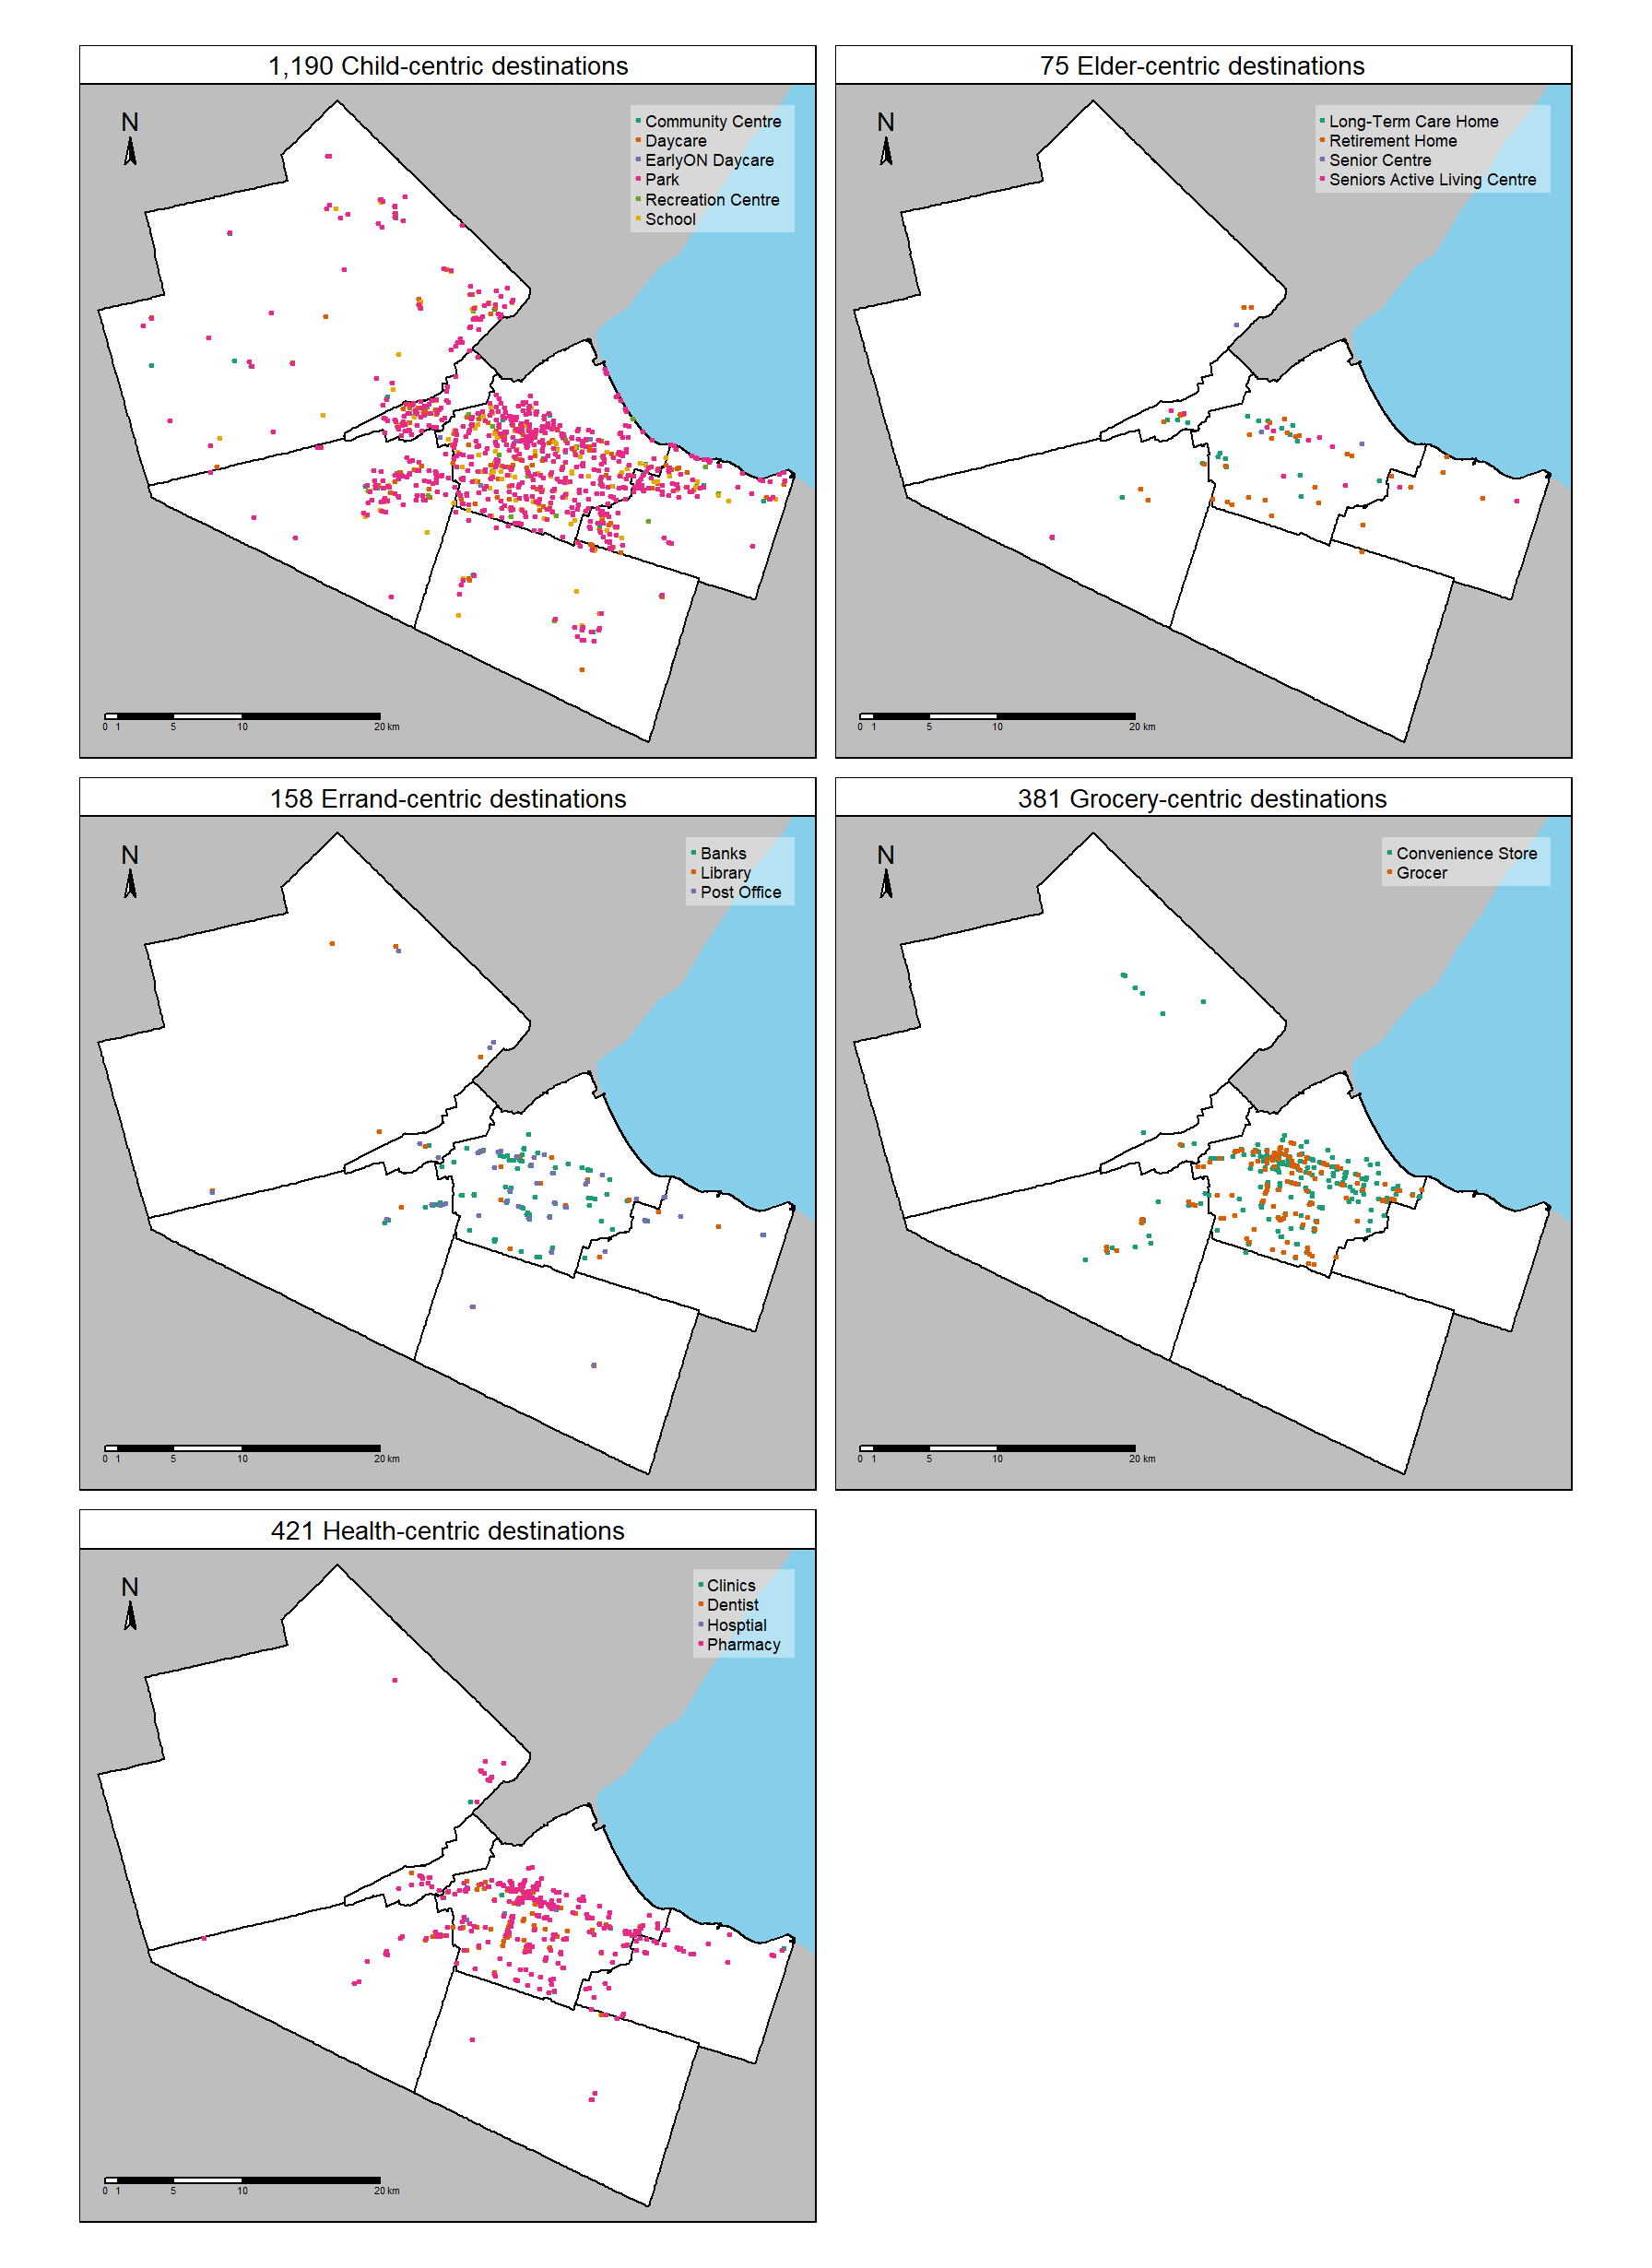
\includegraphics[width=6.25in,height=\textheight]{figures/Fig2-plot_care_categories.png}

}

\caption{\label{fig-Fig2}The geo-located points of care destinations in
the City of Hamilton separated by the author-generated categories of:
child-, elder-, errand-, grocery- and health- centric care categories.
Locations of these destinations were retrieved through multiple sources
as described in the text. Basemap shapefiles are sourced from the Open
Data Hamilton Portal \citep{opendatahamiltonCityBoundary2023} and the
USGS \citep{greatlakesUSGS2010}.}

\end{figure}

For the purpose of this analysis and in absence of city-wide household
preferences for care destinations, all locations are re-weighted to make
each of the six categories conceptually equivalent i.e., each location
within each category \(c\) is weighted to equal
\(O_c = \frac{1}{\sum_{c=1}^{6} c}\frac{\sum_{c=1}^{6} J_c}{J_c}\) where
\(J_c\) is the number of locations within a category \(c\). If this was
not done, the results would favour access to child-centric destinations
as they make up the majority of the dataset. Accessibility literature
has weighted destinations (amenities) using a variety of method such as
estimated capacity of destinations
\citep{liMeasuringMultiactivities2024} or origin-destination flows from
travel surveys
\citep{graellsCityCitiesMeasuring2021, chengInvestigatingWalkingAccessibility2019}.
This work's focus is on household-serving care destinations, so many
destinations do not have traditional `capacities' like health care
facilities have beds. Origin-destination flows to all care destinations
also have not been counted within the TTS
\citep{transportationtomorrowsurvey2018}. So, in this analysis, the five
care categories are re-weighted to represent one-fifth of the dataset.
Conceptually, this simplistic re-weight assumes the population
potentially interacts with all categories and all locations within each
category equally. In absence of empirical data for amenity weight
calibration, this methodological assumption is a limitation.

\begin{itemize}
\tightlist
\item
  Child-centric (1190 destinations each at 0.3739496),
\item
  Elder-centric (75 destinations each at 5.9333333),
\item
  Errand-centric (158 destinations each at 2.8164557),
\item
  Grocery-centric (381 destinations each at 1.167979) and,
\item
  Health- centric (421 destinations each at 1.0570071) .
\end{itemize}

\hypertarget{population-data}{%
\subsection{Population data}\label{population-data}}

To supplement the care destination dataset and complete the
accessibility calculation, population data for the City of Hamilton is
sourced from the 2021 Canadian census using the \{cancensus\} R Package
\citep{governmentofcanadaCensusPopulation2023, vonbergmannCancensusCensusMapper2021}.
Three categories of variables are selected: the population, the percent
of after-tax low-income-cut-off (LICO-AT), and the primary commute mode
used. LICO-AT is a composite indicator included in the census that
reflects the proportion of households spending 20\% more than the area
average on food, shelter and clothing
\citep{governmentofcanadaLowIncomeCutoffs2023}. All data was sourced at
the most granual level of spatial resolution publicly available, the
level of the dissemination area (DA).

Figure~\ref{fig-Fig3} displays the spatial distribution of the total
population and the prevalence of LICO-AT as a percentage of the total
population. Of note is the density of population within Hamilton-Central
(oranges) and the cluster of high density and high LICO-AT prevalence
near the shoreline in Hamilton-Central (dark purple-oranges).

\begin{figure}

{\centering 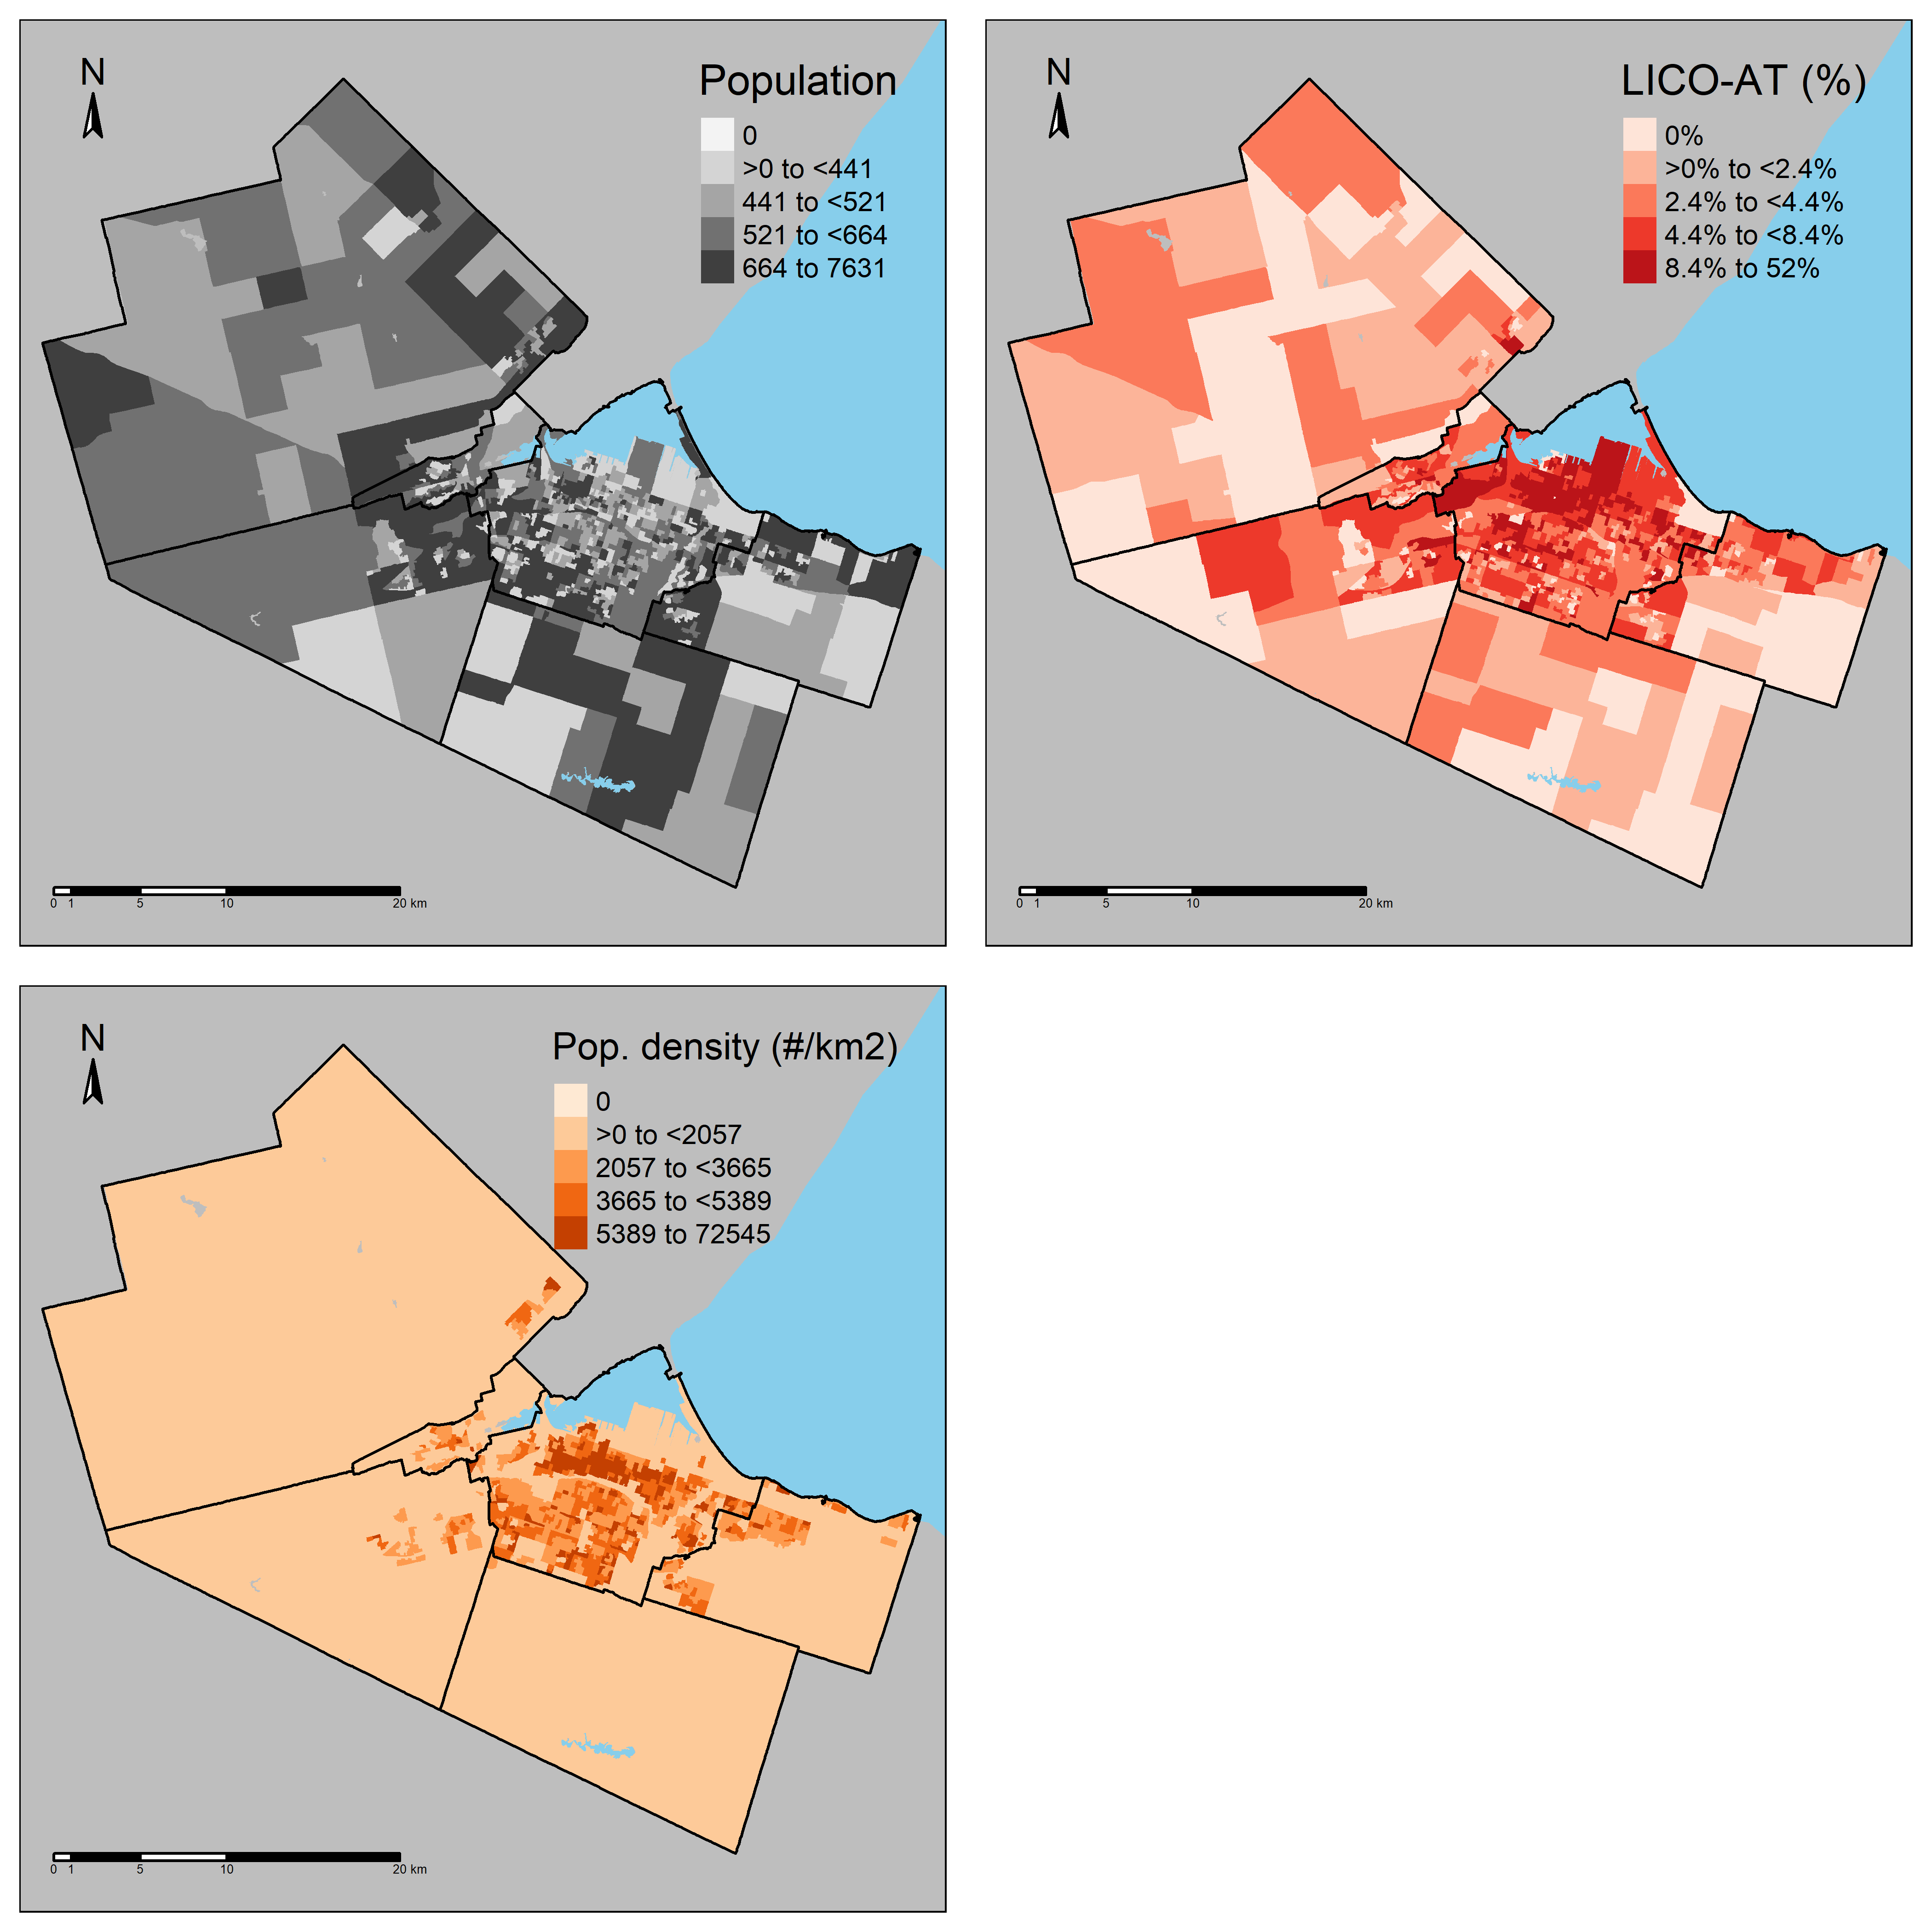
\includegraphics[width=6.25in,height=\textheight]{figures/Fig3-plot_pops.png}

}

\caption{\label{fig-Fig3}The total population in each dissemination area
(DA), visualized with the six former muncipal boundaries in the city of
Hamilton. The left plot represents the population and the right
represents the population density versus the low-income cutt-off after
taxes (LICO-AT) as a percentage of the total DA population. LICO-AT is a
measure of economic disadvantage. The legend categories represent
quartiles. Basemap shapefiles are retrieved from the 2021 Canadian
census \citep{governmentofcanadaCensusPopulation2023}, the Open Data
Hamilton Portal \citep{opendatahamiltonCityBoundary2023} and the USGS
\citep{greatlakesUSGS2010}.}

\end{figure}

Further, the population proportion that commutes by a specific mode
(car, transit, walk, or cycle/other) is visualised in
Figure~\ref{fig-Fig4}. Though mode-choice used in travel to work is not
necessarily reflective of the mode used to travel to care destinations,
to our knowledge no other data is available at a granular level
City-wide that centers mobility of care. The population generally
commutes by car (50\% or higher, is yellow to green), even within the
more densely populated Hamilton-Central. However, for transit and
walking, a group of DAs near the shoreline within Hamilton-Central have
the highest proportion of transit users and those who walk to work
(yellows in the plots that are otherwise red i.e., below 15\%). Those
same DAs are also relatively dense and have a high prevalence of LICO-AT
(Figure~\ref{fig-Fig3}).

\begin{figure}

{\centering 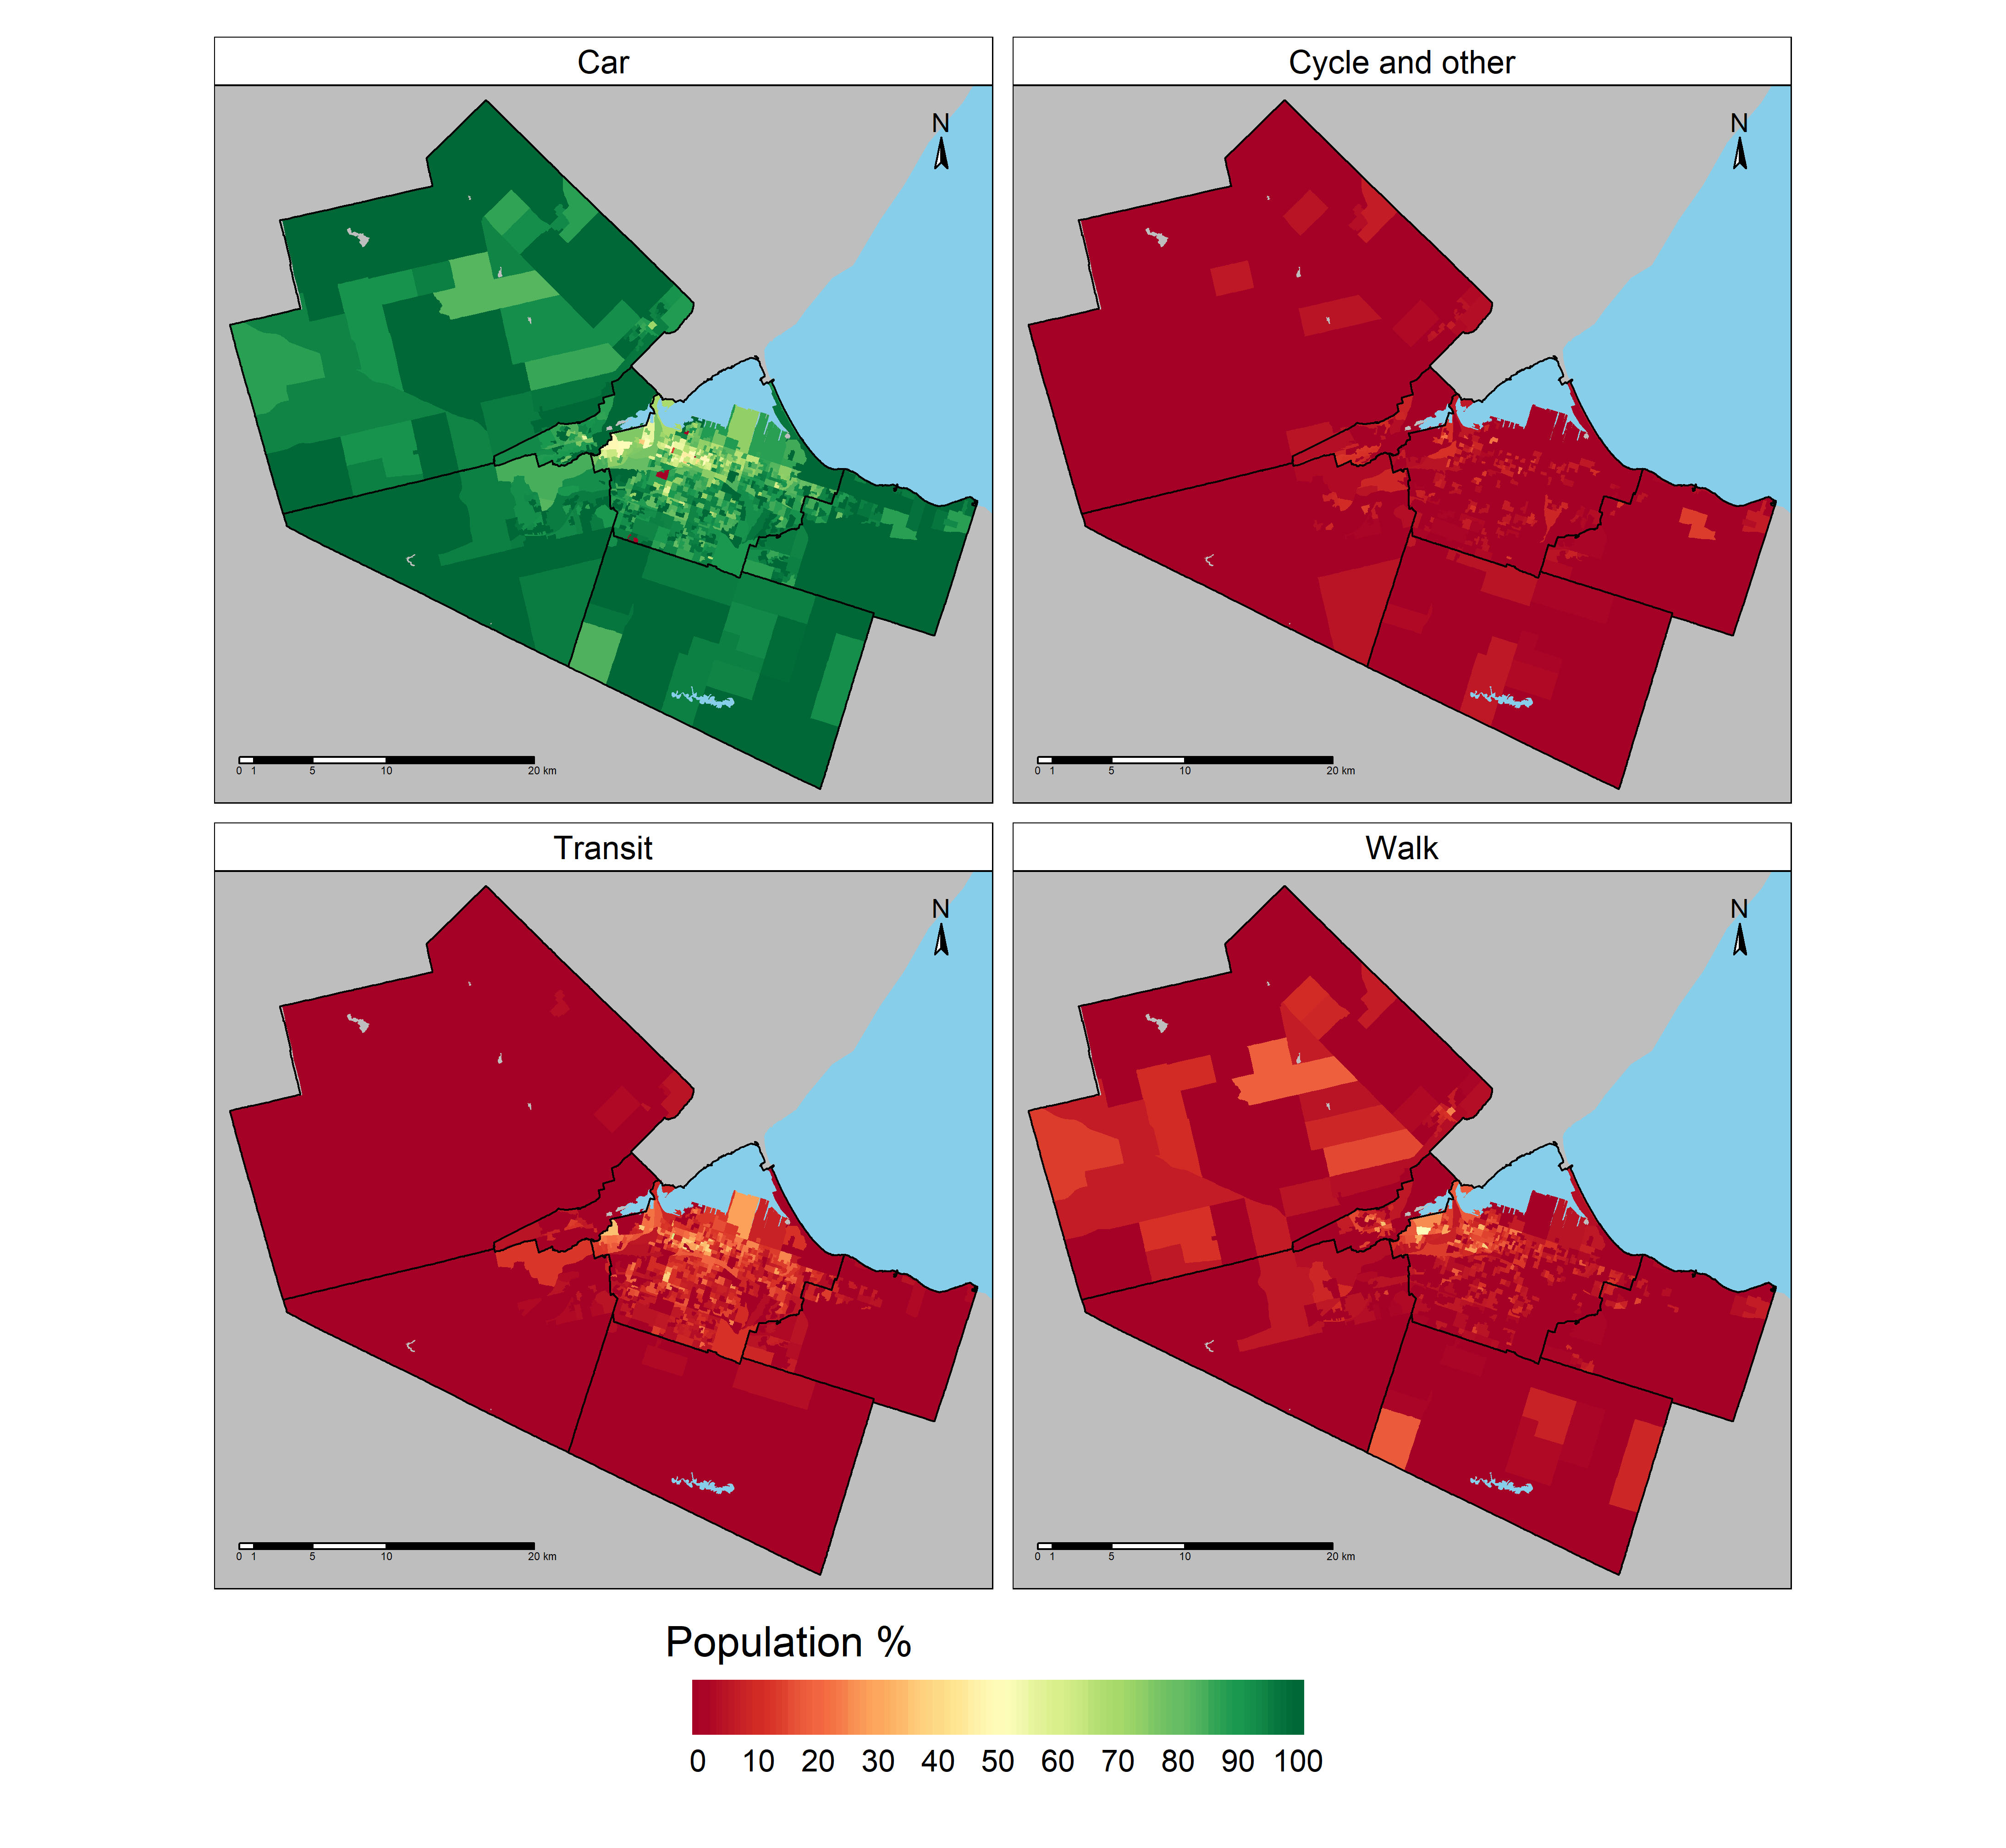
\includegraphics[width=6.25in,height=\textheight]{figures/Fig4-plot_modal_splits.png}

}

\caption{\label{fig-Fig4}The proportion of mode type used for commuting
(aged 15 and older employed in the labour force) in each dissemination
area (DA) as provided by the 2021 Canadian census. Basemap shapefiles
are retrieved from the 2021 Canadian census
\citep{governmentofcanadaCensusPopulation2023}, the Open Data Hamilton
Portal \citep{opendatahamiltonCityBoundary2023} and the USGS
\citep{greatlakesUSGS2010}.}

\end{figure}

\hypertarget{multimodal-travel-time-estimations-and-accessibility-measures}{%
\subsection{Multimodal travel time estimations and accessibility
measures}\label{multimodal-travel-time-estimations-and-accessibility-measures}}

As empirical travel behaviour to care-oriented destinations is
uncounted, it is approximated in the estimation of travel time to all
locations. Travel times by walking, cycling, transit and car is
calculated for each DA to the destination point using the
`travel\_time\_matrix()' function from the \{r5r\} package
\citep{pereiraR5rRapidRealistic2021}. Inputs are point locations of
origins, destinations, an OpenStreetMap road network
\citep{geofabrikOntarioCanadaOpen2023}, and city GTFS transit
routes/schedules \citep{transitfeedsHamiltonStreetRailway2023}. The
origin of each DA and destination location is assumed to be its
geometric centroid. For all modes, travel times under 60 minutes based
on the shortest travel-time path are calculated.

For transit and cycling, additional parameters were included. For
transit travel times, a Wednesday departure time of 8:00AM was selected
\citep{boisjolyDailyFluctuationsTransit2016} with a departure travel
window parameter of \(\pm\) 30 mins. Travel times are calculated for
each minute of the travel window (7:30-8:30AM) and the 25th percentile
from the distribution of travel window times were selected to represent
each origin-destination. Selecting a sufficiently wide window is an
important consideration as travel times are sensitive to transit vehicle
frequency and connecting transfers (see discussion of the modifiable
temporal unit problem e.g.,
\citep{pereiraFutureAccessibilityImpacts2019}). The 25th percentile
indicates that 25\% of trips from that origin to destination have a
travel time that is that length or shorter. This assumption provides an
optimistic perspective of transit travel times. For cycling travel
times, level 1 or 2 traffic level of stress routes (i.e., dedicated or
separated cycling lanes respectively) were selected. The level of
traffic stress is a variable associated with links of the OSM road
network; level 1 and 2 are considered the default.

The \textbf{cumulative opportunity} and \textbf{spatial availability}
measures are used to estimate the potential access to care that each
mode provides to the DA. From the cumulative opportunity measure, the DA
level values represent the potential interaction with reachable
destinations a population located at DA could access using a given mode.
The interpretation of the spatial availability measure is different:
each DA level values are a proportional value of all the care
destinations in Hamilton. Each proportional value represents the
potential availability of reachable care destinations to a mode-using
population located at the DA.

\textbf{Cumulative opportunity accessibility}: takes the following
general form for multi-modal calculation: \[
S_i^m=\sum_{j}O_j\cdot f^m(c_{ij}^m)
\] \noindent Where:

\begin{itemize}
\tightlist
\item
  \(i\) is a set of origin locations.
\item
  \(j\) is a set of destination locations.
\item
  \(m\) is a set of modes.
\item
  \(O_j\) is a number of opportunities at \(j\), in our case weighted.
\item
  \(c_{ij}^m\) is the travel cost between \(i\) and \(j\) for each
  \(m\).
\item
  \(f^m(\cdot)\) is an impedance function of \(c^m_{ij}\) for each
  \(m\); within the cumulative opportunity approach, it is a binary
  function that takes the value of 1 if \(c^m_{ij}\) is less than a
  selected value \citep{handyMeasuringAccessibilityExploration1997}.
\item
  \(S^m_{i}\) is the unconstrained accessibility for \(m\) at each
  \(i\).
\end{itemize}

\textbf{Spatial availability}, on the other hand, takes the following
general form for multi-modal calculation: \[
V^m_{i} = \sum_{j} O_j\ F^{tm}_{ij}
\] \noindent Where:

\begin{itemize}
\tightlist
\item
  \(i\), \(j\), and \(m\) is a set of origin locations, destination
  locations, and modes respectively.
\item
  \(O_j\) is a number of opportunities at \(j\), in our case weighted.
\item
  \(F^{tm}_{ij}\) is a balancing factor for each \(m\) at each \(i\). It
  depends on the size of the populations at different locations that
  demand opportunities \(O_j\), as well as the cost of movement in the
  system \(f(c_{ij})\).
\item
  \(V^m_{i}\) is the constrained accessibility (spatial availability)
  for \(m\) at each \(i\); the sum of \(V^m_{i}\) for all \(m\) at each
  \(i\) is equivalent to the total sum of opportunities in the region
  (i.e., \(\sum_j O_j = \sum_i V_i = \sum_{m} \sum_{i} V^m_{i}\)).
\end{itemize}

What makes spatial availability stand apart from other competitive
measures is the multimodal balancing factor \(F^{tm}_{ij}\)
\citep[see][]{soukhovMultimodalSpatialAvailability2023, soukhovIntroducingSpatialAvailability2023}.
\(F^{tm}_{ij}\) implements a proportional allocation mechanism that
ensures the sum of all spatial availability values at each \(i\) always
matches the total number of opportunities in the region. \(F^{tm}_{ij}\)
consists of two parts: the first is a population-based proportional
allocation factor \(F_i^{pm}\) that models the mass effect (relative
population-demand for opportunities) and the second is an
impedance-based proportional allocation factor \(F_{ij}^{cm}\) that
models the cost effect (relative travel time). Both factors consider
competition through proportional allocation: \(F^{pm}_{i}\) estimates a
proportion of how many people are in each \(i\) and using each \(m\)
relative to the region and \(F^{cm}_{ij}\) estimates a proportion of the
cost of travel from \(i\) to \(j\) at each \(i\) using each \(m\)
relative to the region. Since \(F^{pm}_{i}\) and \(F^{mc}_{i}\) are
proportions, \(\sum_{m}\sum_{i}F^{pm}_{i} = 1\) and
\(\sum_{m} \sum_{i}F^{cm}_{i}=1\). Both factors are combined to create
the total balancing factor \(F^{tm}_{ij}\) used to calculate \(V^m_i\):

\[
F^{tm}_{ij} = \frac{F^{pm}_{i} \cdot F^{cm}_{ij}}{\sum_{m} \sum_{i} F^{pm}_{i} \cdot F^{cm}_{ij}}
\] \noindent Where:

\begin{itemize}
\tightlist
\item
  The factor for allocation by population for each \(m\) at each \(i\)
  is \(F^{pm}_{i} = \frac{P_{i}^m}{\sum_{m}\sum_{i} P_{i}^m}\). This
  factor makes opportunities available based on demand.
\item
  The factor for allocation by cost of travel for each \(m\) at \(i\) is
  \(F_{ij}^{cm} = \frac{f^m(c_{ij}^m)}{\sum_{m} \sum_{i} f^m(c_{ij}^m)}\).
  This factor makes opportunities available preferentially to those who
  can reach them at a lower cost.
\end{itemize}

The travel impedance threshold used in both measures is 15 minutes and
30 minutes; each measure is calculated eight times, once for each four
modes and assuming a travel time cut-off of 15 minutes or less and
another assuming a travel time cut-off of 30 minutes or less. The
selection of travel time thresholds is informed by the literature. Only
one study to date has calculated the average travel time to all
different categories of care destinations (16 minutes by car and 36 by
public transport) \citep{ravensbergenExploratoryAnalysisMobility2022}.
Other literature typically considers trips to one type of care category
(e.g., health, or school, or grocery stores) Here, travel times vary by
care category (e.g., 15 minutes to grocery shopping
\citep{hamrickTimeCostAccess2012} or 20.45 for cancer treatments
\citep{segelRuralurbanDifferencesAssociation2020}. In other care-related
accessibility analyses, time-cut offs include 10 mins (for daycares)
\citep{fransenCommuterbasedTwostepFloating2015} and 30 mins to 1 hr (for
hospitals) \citep{schuurmanDefiningRationalHospital2006}. 15 and 30
minutes were selected to broadly reflect this past research. The use of
a binary travel time threshold, as opposed to more complex impedance
functions, was selected to simplify communication of assumed travel
behaviour. As mentioned, lacking region-specific empirical data
regarding care-centric travel, this work establishes a methodology to
streamline access to care interpretation and analysis for when that data
is available.

This work uses both constrained and unconstrained accessibility measures
to elucidate different interpretations of access to care. As an
unconstrained measure, cumulative opportunity measure counts all the
destinations that can be reached from each DA within a travel cost, for
each DA. From a region-wide perspective, a destination that can be
reached is counted multiple times by all DAs that can reach it, so the
sum of all cumulative opportunity DA values in the region is not
meaningful. Simply, if walking-mode provides access to some number of
opportunities within a 30 minutes, car-mode provides some greater access
within 30 minutes, and the access that walk-mode is not discounted by
the population using car-mode and the greater number of opportunities
they can potentially access. However, cumulative opportunity measure is
intuitive to implement, a part in why it has been widely adopted in
accessibility research and considered a introductory method to more
advanced accessibility measure
\citep{elgeneidyMakingAccessibilityWork2021}.

On the other hand, spatial availability is constrained accessibility
measure that considers competition
\citep{soukhovIntroducingSpatialAvailability2023}. It incorporates the
concept of the \emph{finite}: opportunities are numbered in the region
so they can be potentially interacted with more or less based on the
travel impedance offered by the zone (i.e., the travel cost on the
transport network) as well as how densely or sparsely the zone is
populated with opportunity-seeking opportunities. This is especially
important considering population-distinct characteristics like selected
travel modes. In a North American context, car-modes can potentially
access more opportunities (unconstrained) because of their higher range
relative to transit. But if opportunities are considered finite, high
car mobility may take-up a higher share of opportunities from
populations using modes that offer lower mobility, especially in zones
where there is a high population and car-using modal split. Cumulative
opportunities does not consider the relative population-demand for care
destinations while spatial availability does: the use of these two
measure illustrates distinct results.

\hypertarget{results}{%
\section{Results}\label{results}}

\hypertarget{unconstrained-access-to-care}{%
\subsection{Unconstrained access to
care}\label{unconstrained-access-to-care}}

The cumulative opportunity accessibility plots for each mode are shown
in Figure~\ref{fig-Fig5}. They visualise an unconstrained count of care
destinations that can be reached by each mode from each DA. The higher
the zonal value, the more potential interaction with care destinations.
This greater potential is conceptualised as a positive outcomes of well
functioning land-use and transport networks
\citep{corderaImpactAccessibilityPublic2019, blumenbergDriveWorkRelationship2017, cuiSpatialAccessPublic2020}.
Spatial trends between the 15-min and 30-min threshold plots are similar
(values are grouped by quantile). Three significant findings between
modes can be identified. First, the access that the car-mode provides is
significantly higher relative to other modes. Travel by car results in
the greatest maximum number of potential interactions to care
destinations (1939 opportunities for 15-min and 2209 opportunities for
30-mins). Next, access by cycling is also relatively high. It provides
the second most opportunities for interactions after travel by car, and
affords at least one opportunity for interaction in more DAs than
walking and transit use. Finally, access by transit is high and walking
is also relatively high within Hamilton-Central but low elsewhere.

\begin{figure}

{\centering 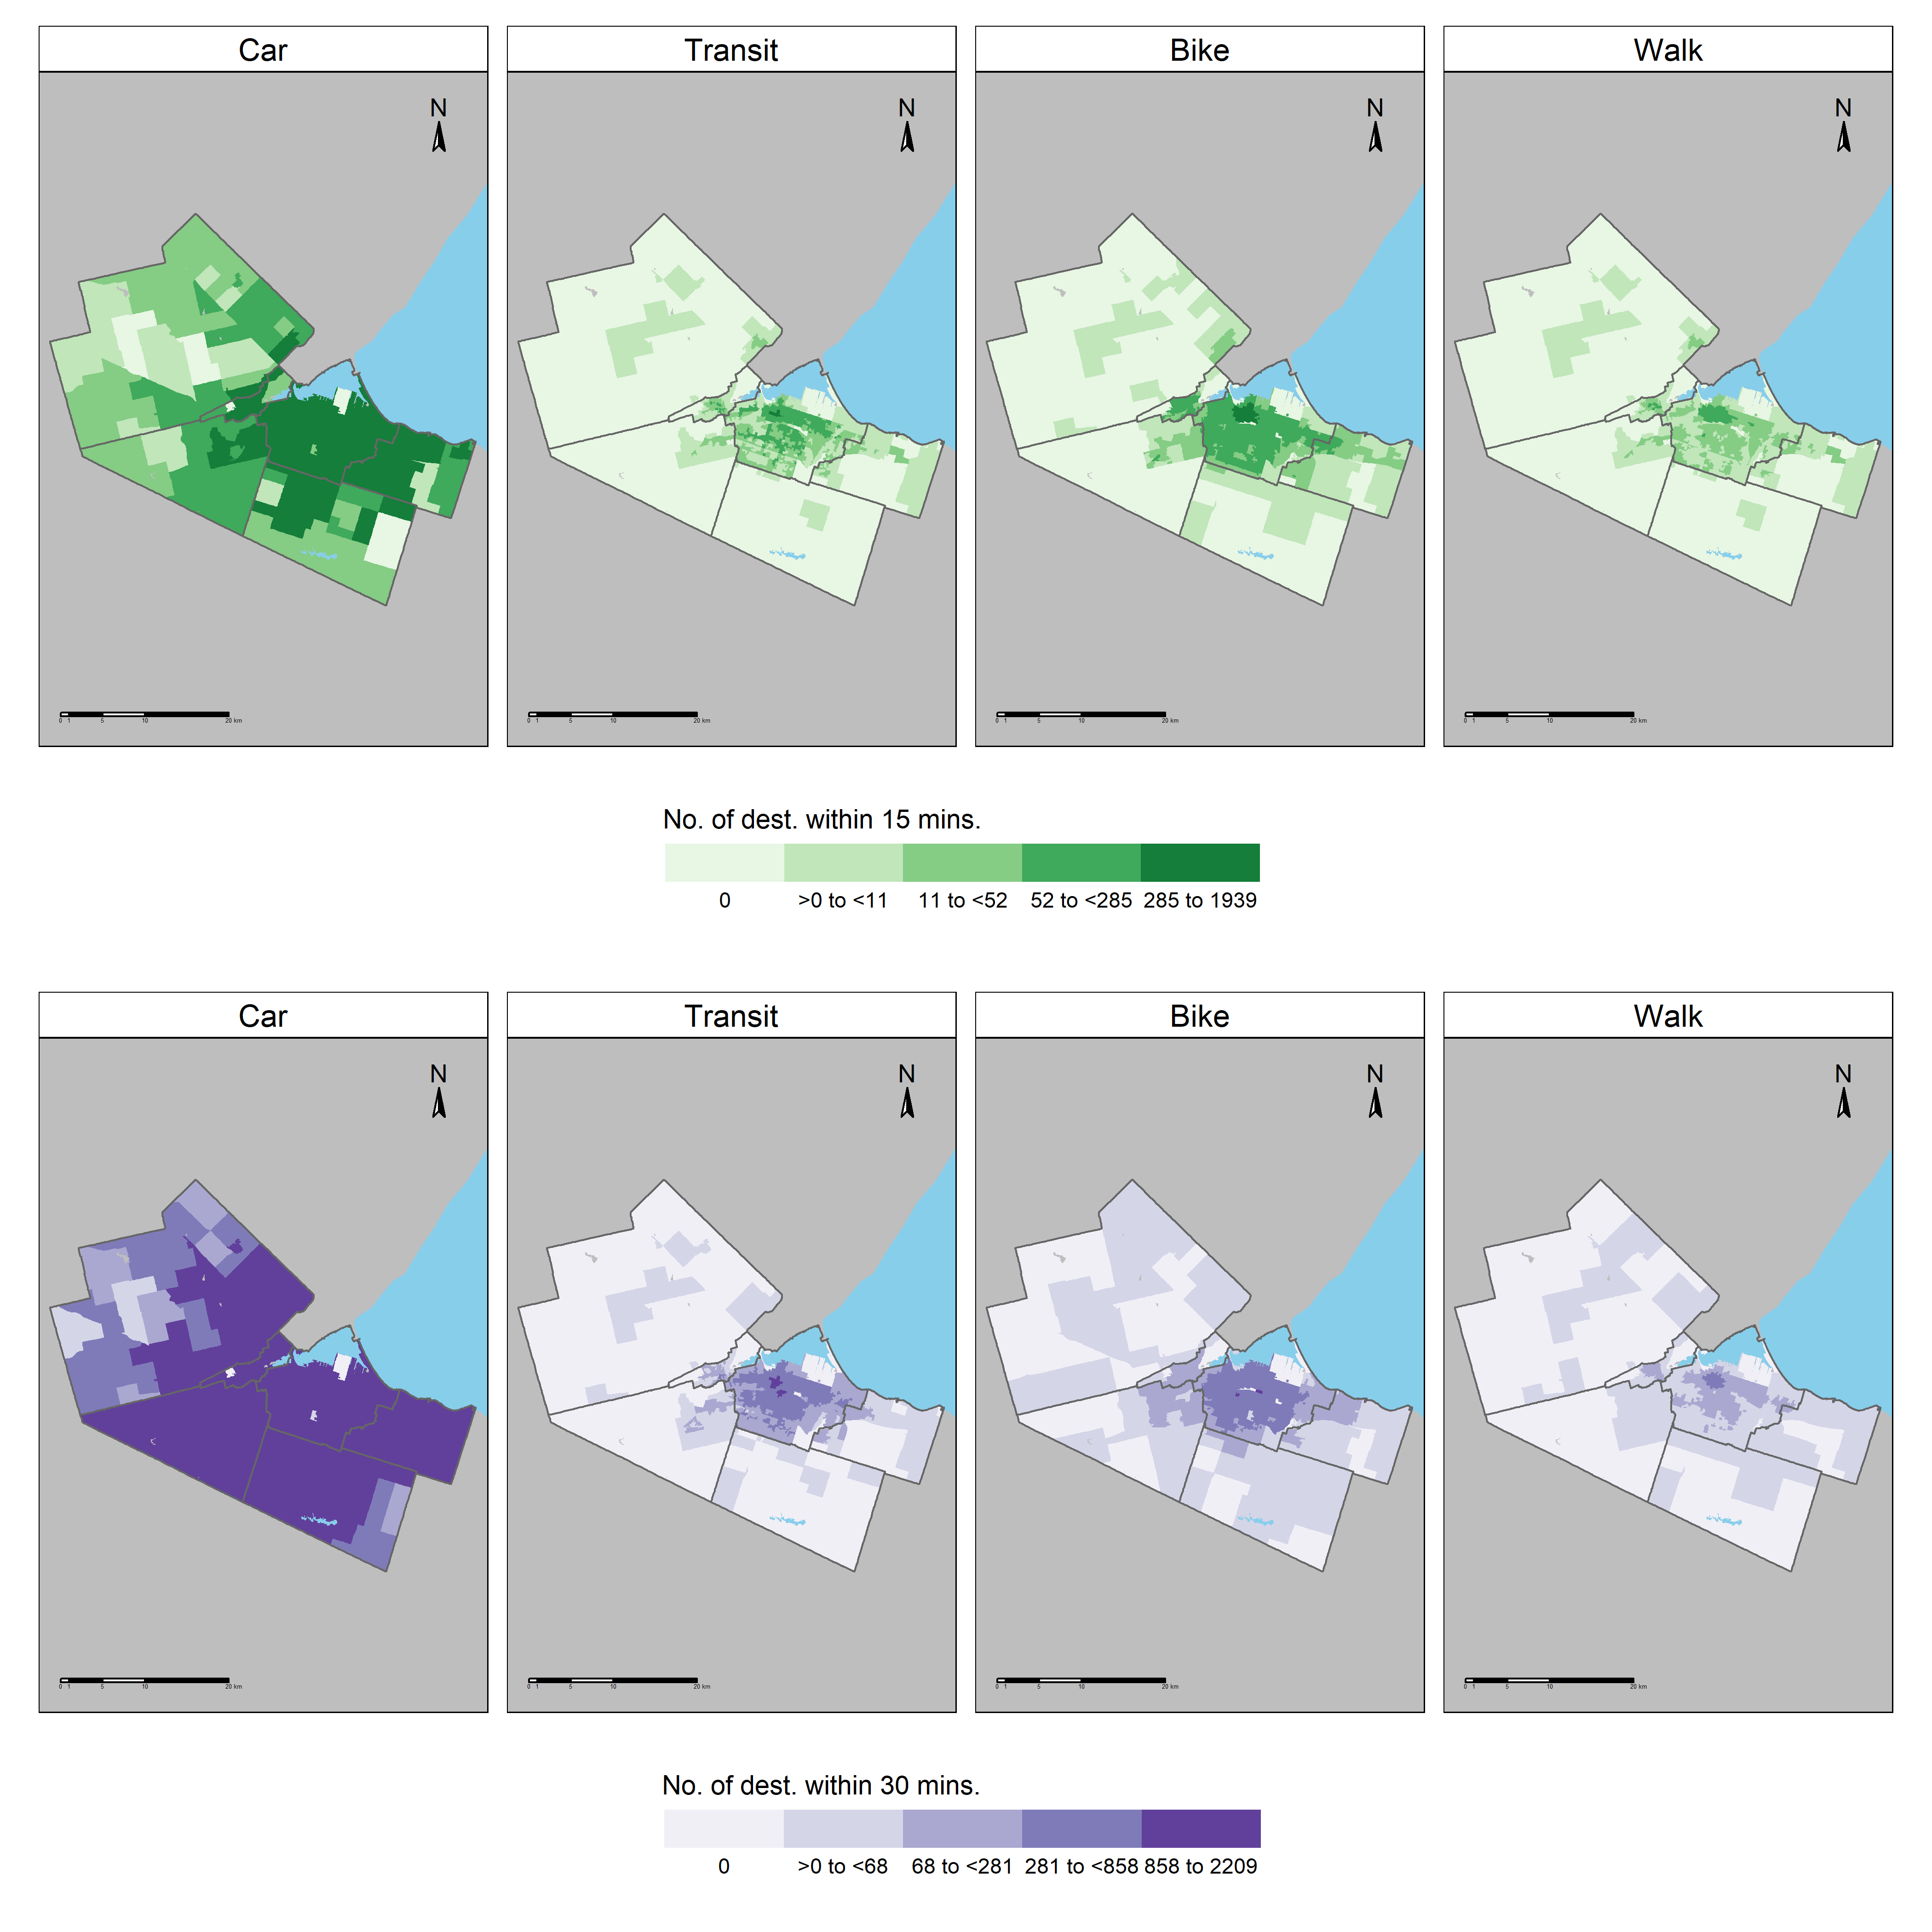
\includegraphics[width=6.25in,height=\textheight]{figures/Fig5-plot_cum_opp_measures.png}

}

\caption{\label{fig-Fig5}The cumulative opportunity measure. The number
of care destinations that can be reached, per DA, within 15 mins (top)
and 30 mins (bottom). Basemap shapefiles are retrieved from the 2021
Canadian census \citep{governmentofcanadaCensusPopulation2023}, the Open
Data Hamilton Portal \citep{opendatahamiltonCityBoundary2023} and the
USGS \citep{greatlakesUSGS2010}.}

\end{figure}

From Figure~\ref{fig-Fig5}, car-mode offering high accessibility to
destinations is an expected outcome given the car-oriented design of
North American cities \citep{saeidizandRevisitingCarDependency2022}.
However, access by non-car modes is great within many DAs in
Hamilton-Central (Q3 and Q4). As well, cycling provides some access to
destinations (Q1) in more rural communities. While car ownership is high
in Hamilton, not everyone has access to a private vehicle: 13\% of
Hamilton households own zero vehicles
\citep{datamanagementgroupTTSTransportationTomorrow2018}. Unconstrained
access is insightful in illustrating the spatial accessibility to
destinations that people may have, but it does not account for how the
overall access provided by the transportation systems to destinations is
allocated to different mode-using populations. This lack of
consideration may conjure misleading conclusions, namely the inflated
promise of lower access-providing modes.

\hypertarget{constrained-acces-to-care}{%
\subsection{Constrained acces to care}\label{constrained-acces-to-care}}

Consider cycling: the access provided by this mode appears promising
when examining the cumulative opportunity results
(Figure~\ref{fig-Fig5}). This may be in part because interpreting
cycling access against the much higher access providing car-mode is
difficult. Unconstrained access by car is high (Q4), but at least
cycling-mode can achieve Q3 levels in Hamilton-Central and Q1 beyond.
However, by conceptualising the amount of accessibility available in the
region as a total, one can answer how many opportunities are available
to those using the cycling-mode considering the allocation to the other
three mode-using populations. This comparison cannot be addressed using
unconstrained accessibility, but can be explored with spatial
availability (constrained accessibility), mapped in
Figure~\ref{fig-Fig6}.

\begin{figure}

{\centering 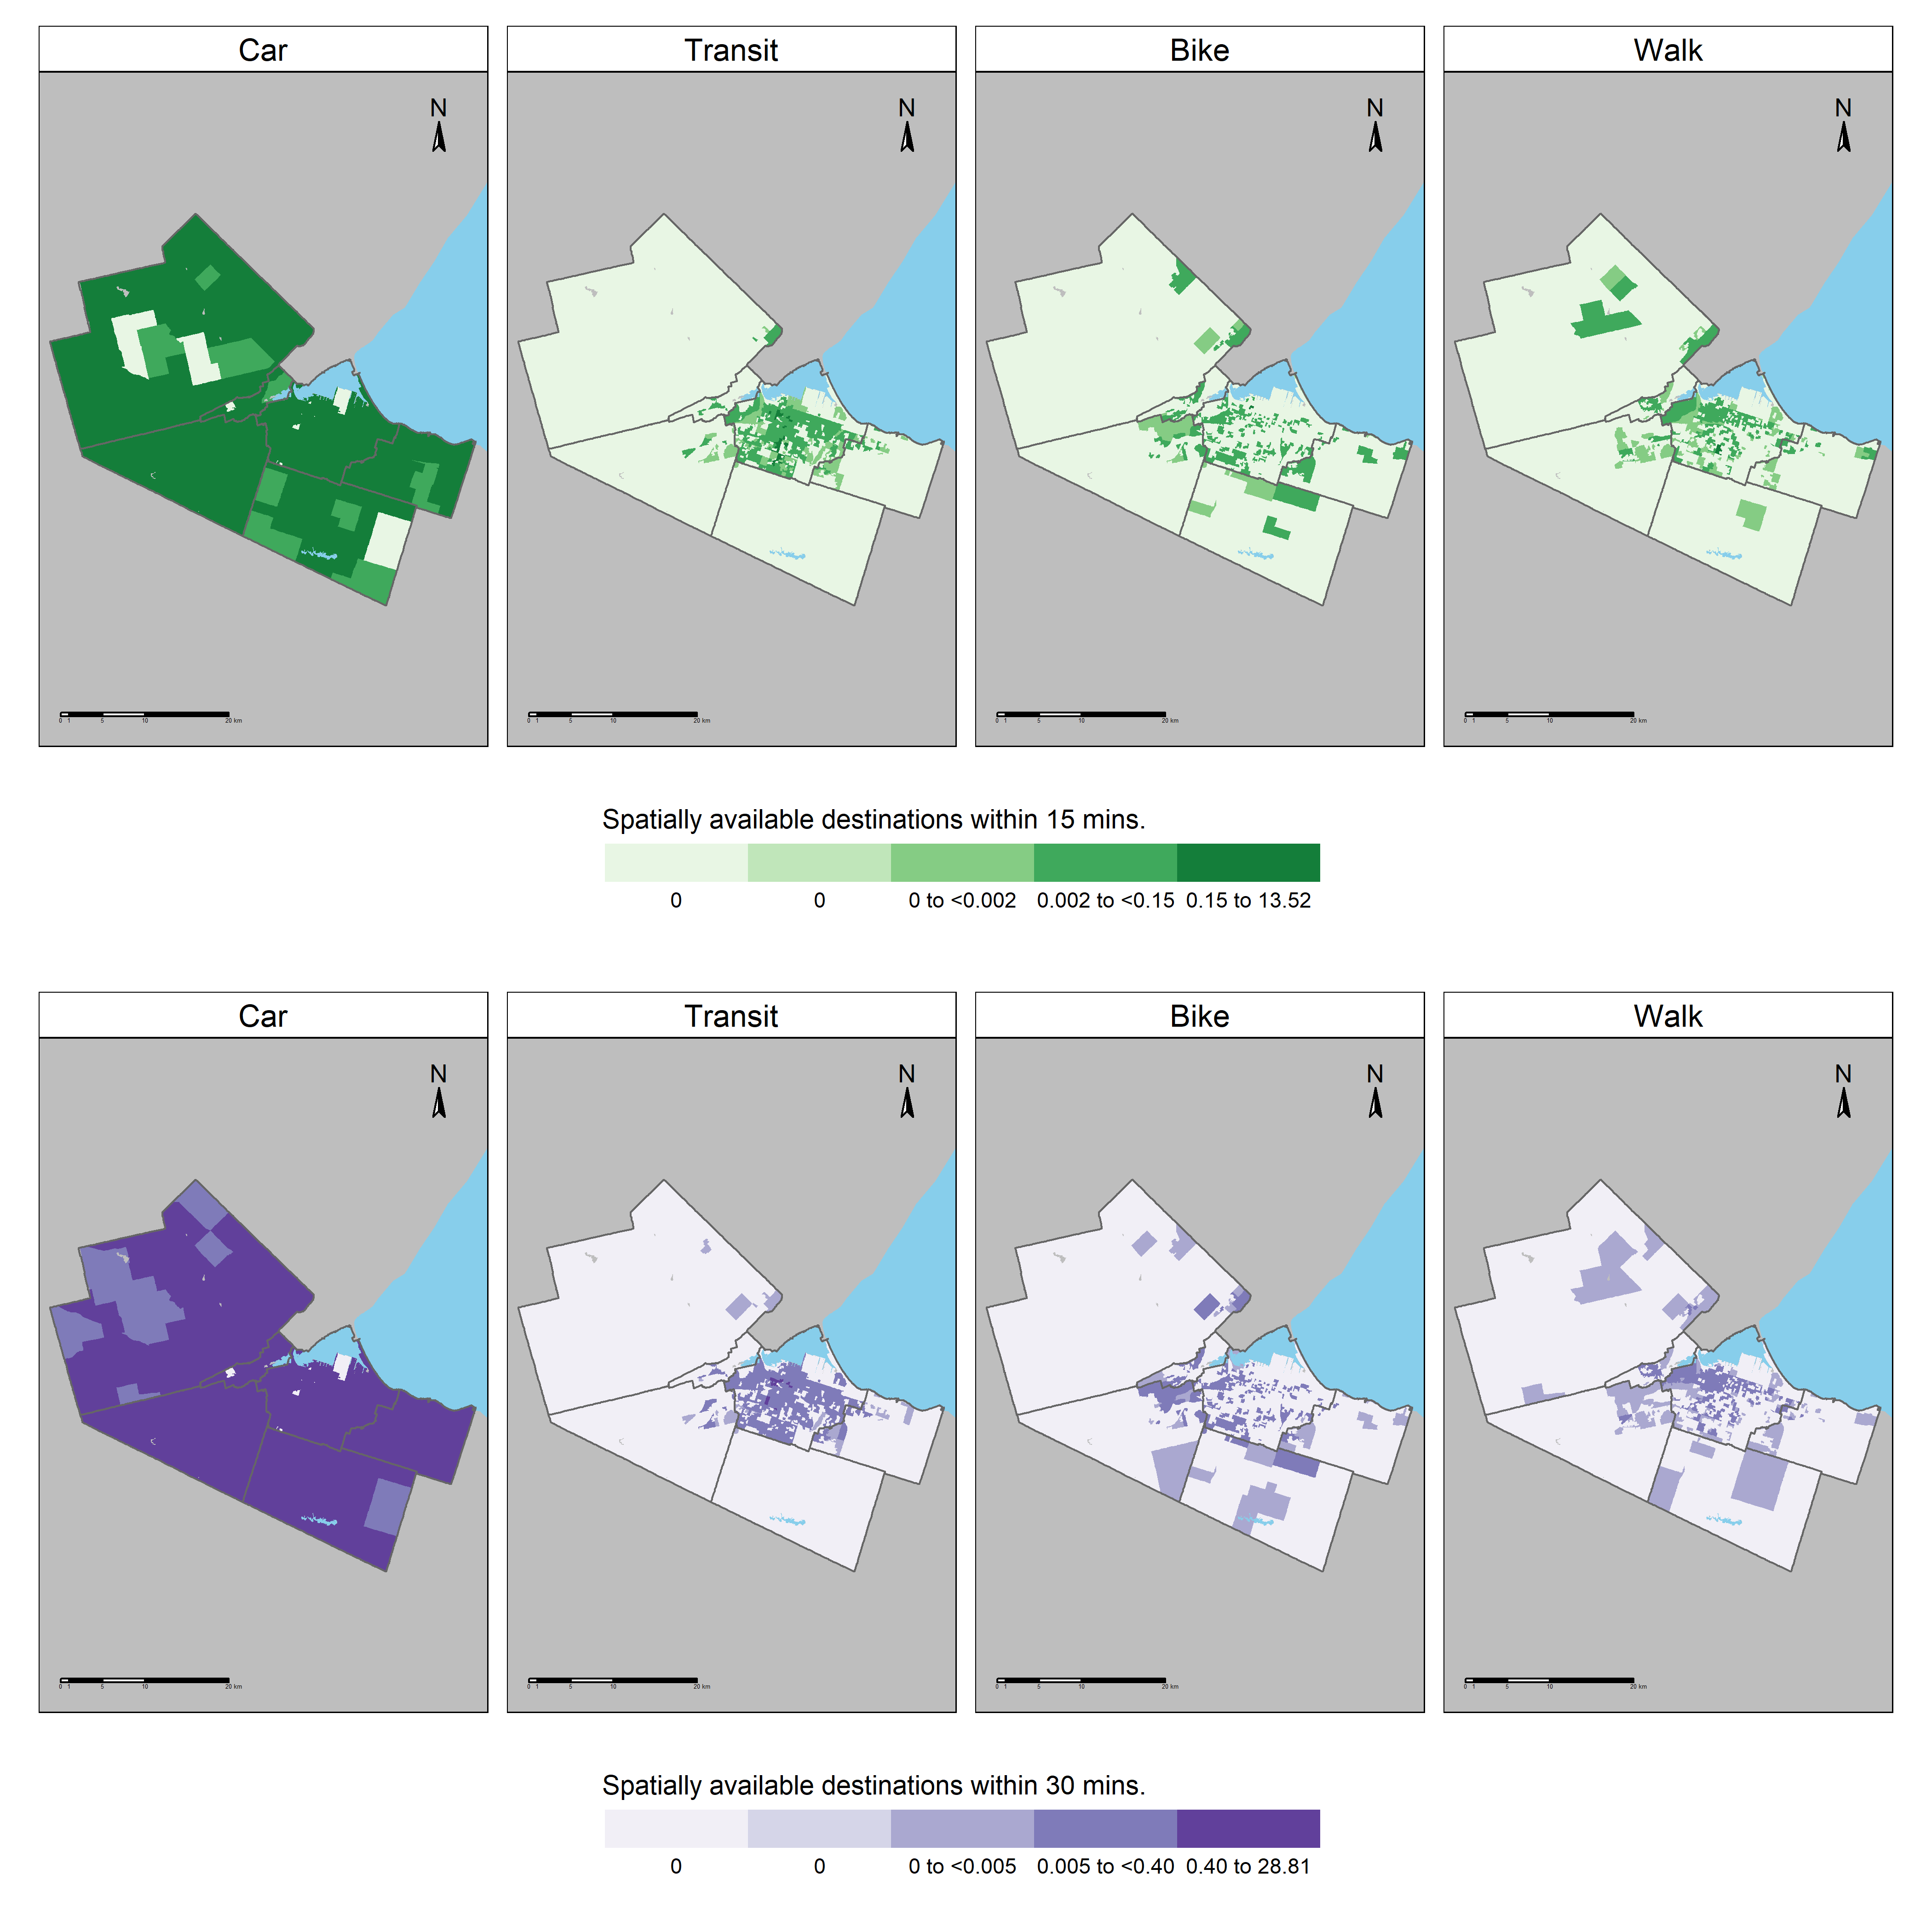
\includegraphics[width=6.25in,height=\textheight]{figures/Fig6-plot_Savail_measures.png}

}

\caption{\label{fig-Fig6}Spatial availability: the number of care
destinations that can be reached, per DA, within 15 mins (top) and 30
mins (bottom). Basemap shapefiles are retrieved from the 2021 Canadian
census \citep{governmentofcanadaCensusPopulation2023}, the Open Data
Hamilton Portal \citep{opendatahamiltonCityBoundary2023} and the USGS
\citep{greatlakesUSGS2010}.}

\end{figure}

This study's calculation of spatial availability (Figure~\ref{fig-Fig6})
assumes population mode-shares (proportions shown in
Figure~\ref{fig-Fig4}), while the unconstrained analysis does not. In
this context, from Figure~\ref{fig-Fig6} it can be observed that those
who use car-modes are allocated the most spatial availability i.e., the
proportion of spatial access to destinations out of all spatial access
to destinations in the region. A similar spatial trend is found in the
unconstrained accessibility analysis (Figure~\ref{fig-Fig5}). However,
since Figure~\ref{fig-Fig6} accounts for the mode-using population, the
results are more rich. Spatial availability for motorists is in-part due
to the exceptionally high proportion of car-using populations
(especially in rural communities) as well as car-mode's relatively
competitive travel time. There is a higher car-using population and the
car-mode has low travel times to destinations allowing the car-mode
using population in each DA to capture the majority of spatial
availability. Figure~\ref{fig-Fig5} only sheds light on how much
unconstrained accessibility the car-mode could potentially provided to
people within a DA.

While the unconstrained accessibility analysis (Figure~\ref{fig-Fig5})
demonstrates that non-car modes are promising in urban areas, as well as
cycling in rural communities, Figure~\ref{fig-Fig6} demonstrates a more
nuanced perspective. Though non-car modes may provide good unconstrained
accessibility within Hamilton-Central (and some access in rural
communities), they do not provide similar levels of spatial
availability. Car-using populations capture more spatial availability,
even in the centre of Hamilton-Central, than all other modes. Note the
lower number of Q3 and Q4 values within and radiating outwards from
Hamilton-Central for non-car modes in Figure~\ref{fig-Fig6} compared to
Figure~\ref{fig-Fig5}. Differences between the two measures follow a
similar descriptive trend for both travel times.

The proportion of spatial availability allocated to a mode-using
population can also be directly compared. This sheds light on what mode,
and in what region, a mode-using population captures more than its equal
share of spatial availability. Overall, 97\% of the spatial availability
is taken by motorists (destinations within 30-minutes) but they only
represent 87\% of the population; they have disproportionately more
availability than their population's presence in the city. They capture
this availability from non-car mode using populations that exists in
high proportions with lower spatial availability (i.e., transit users to
destinations within 30-minutes are 7\% of the population but take 2\% of
the spatial availability, 30-minute cyclist are 2\% of the population
but represent 0.3\% of the spatial availability, and 30-minute walkers
are 4\% of the population but are allocated 0.3\% of the spatial
availability.

The key interpretation from Figure~\ref{fig-Fig6} is that if certain
modes capture an exceptional proportion of availability, than the
availability left for other modes is lower overall. This does not
necessarily have to align with the unconstrained accessibility that mode
offers. As noted, non-car modes have the potential to offer higher
unconstrained access (within Hamilton-Central) in Figure~\ref{fig-Fig5}.
But as it exists (assuming modal commute shares), the majority of
spatial availability to care destinations can still be captured by
motorists even in DAs where car mode share is under 50\% (such as
Hamilton-Central, see proportions in Figure~\ref{fig-Fig4}).

\hypertarget{equity-considerations}{%
\subsection{Equity considerations}\label{equity-considerations}}

To draw insights on who may reside in DAs where populations are
advantaged with higher modal spatial availability, a cross-tabulation of
low-high spatial availability \& LICO-AT prevalence and high-no spatial
availability \& LICO-AT prevalence is visualised in
Figure~\ref{fig-Fig8}. The modal spatial availability is divided by the
mode-using population in each DA, resulting in the rate of modal spatial
availability. LICO prevalence is the proportion of population that falls
below the LICO-AT (see Figure~\ref{fig-Fig3}). Figure~\ref{fig-Fig8} can
be interpreted as follows: residents who use a specific mode in a
``yellow'' DA reside in a DA that offers below average spatial
availability (i.e., below or equal to the the 50th percentile (median)
levels of spatial availability per mode-using population) and the
population within the DA has a high LICO-prevalence (i.e, 80th
percentile or higher (8.4\% or more)).

\begin{figure}

{\centering 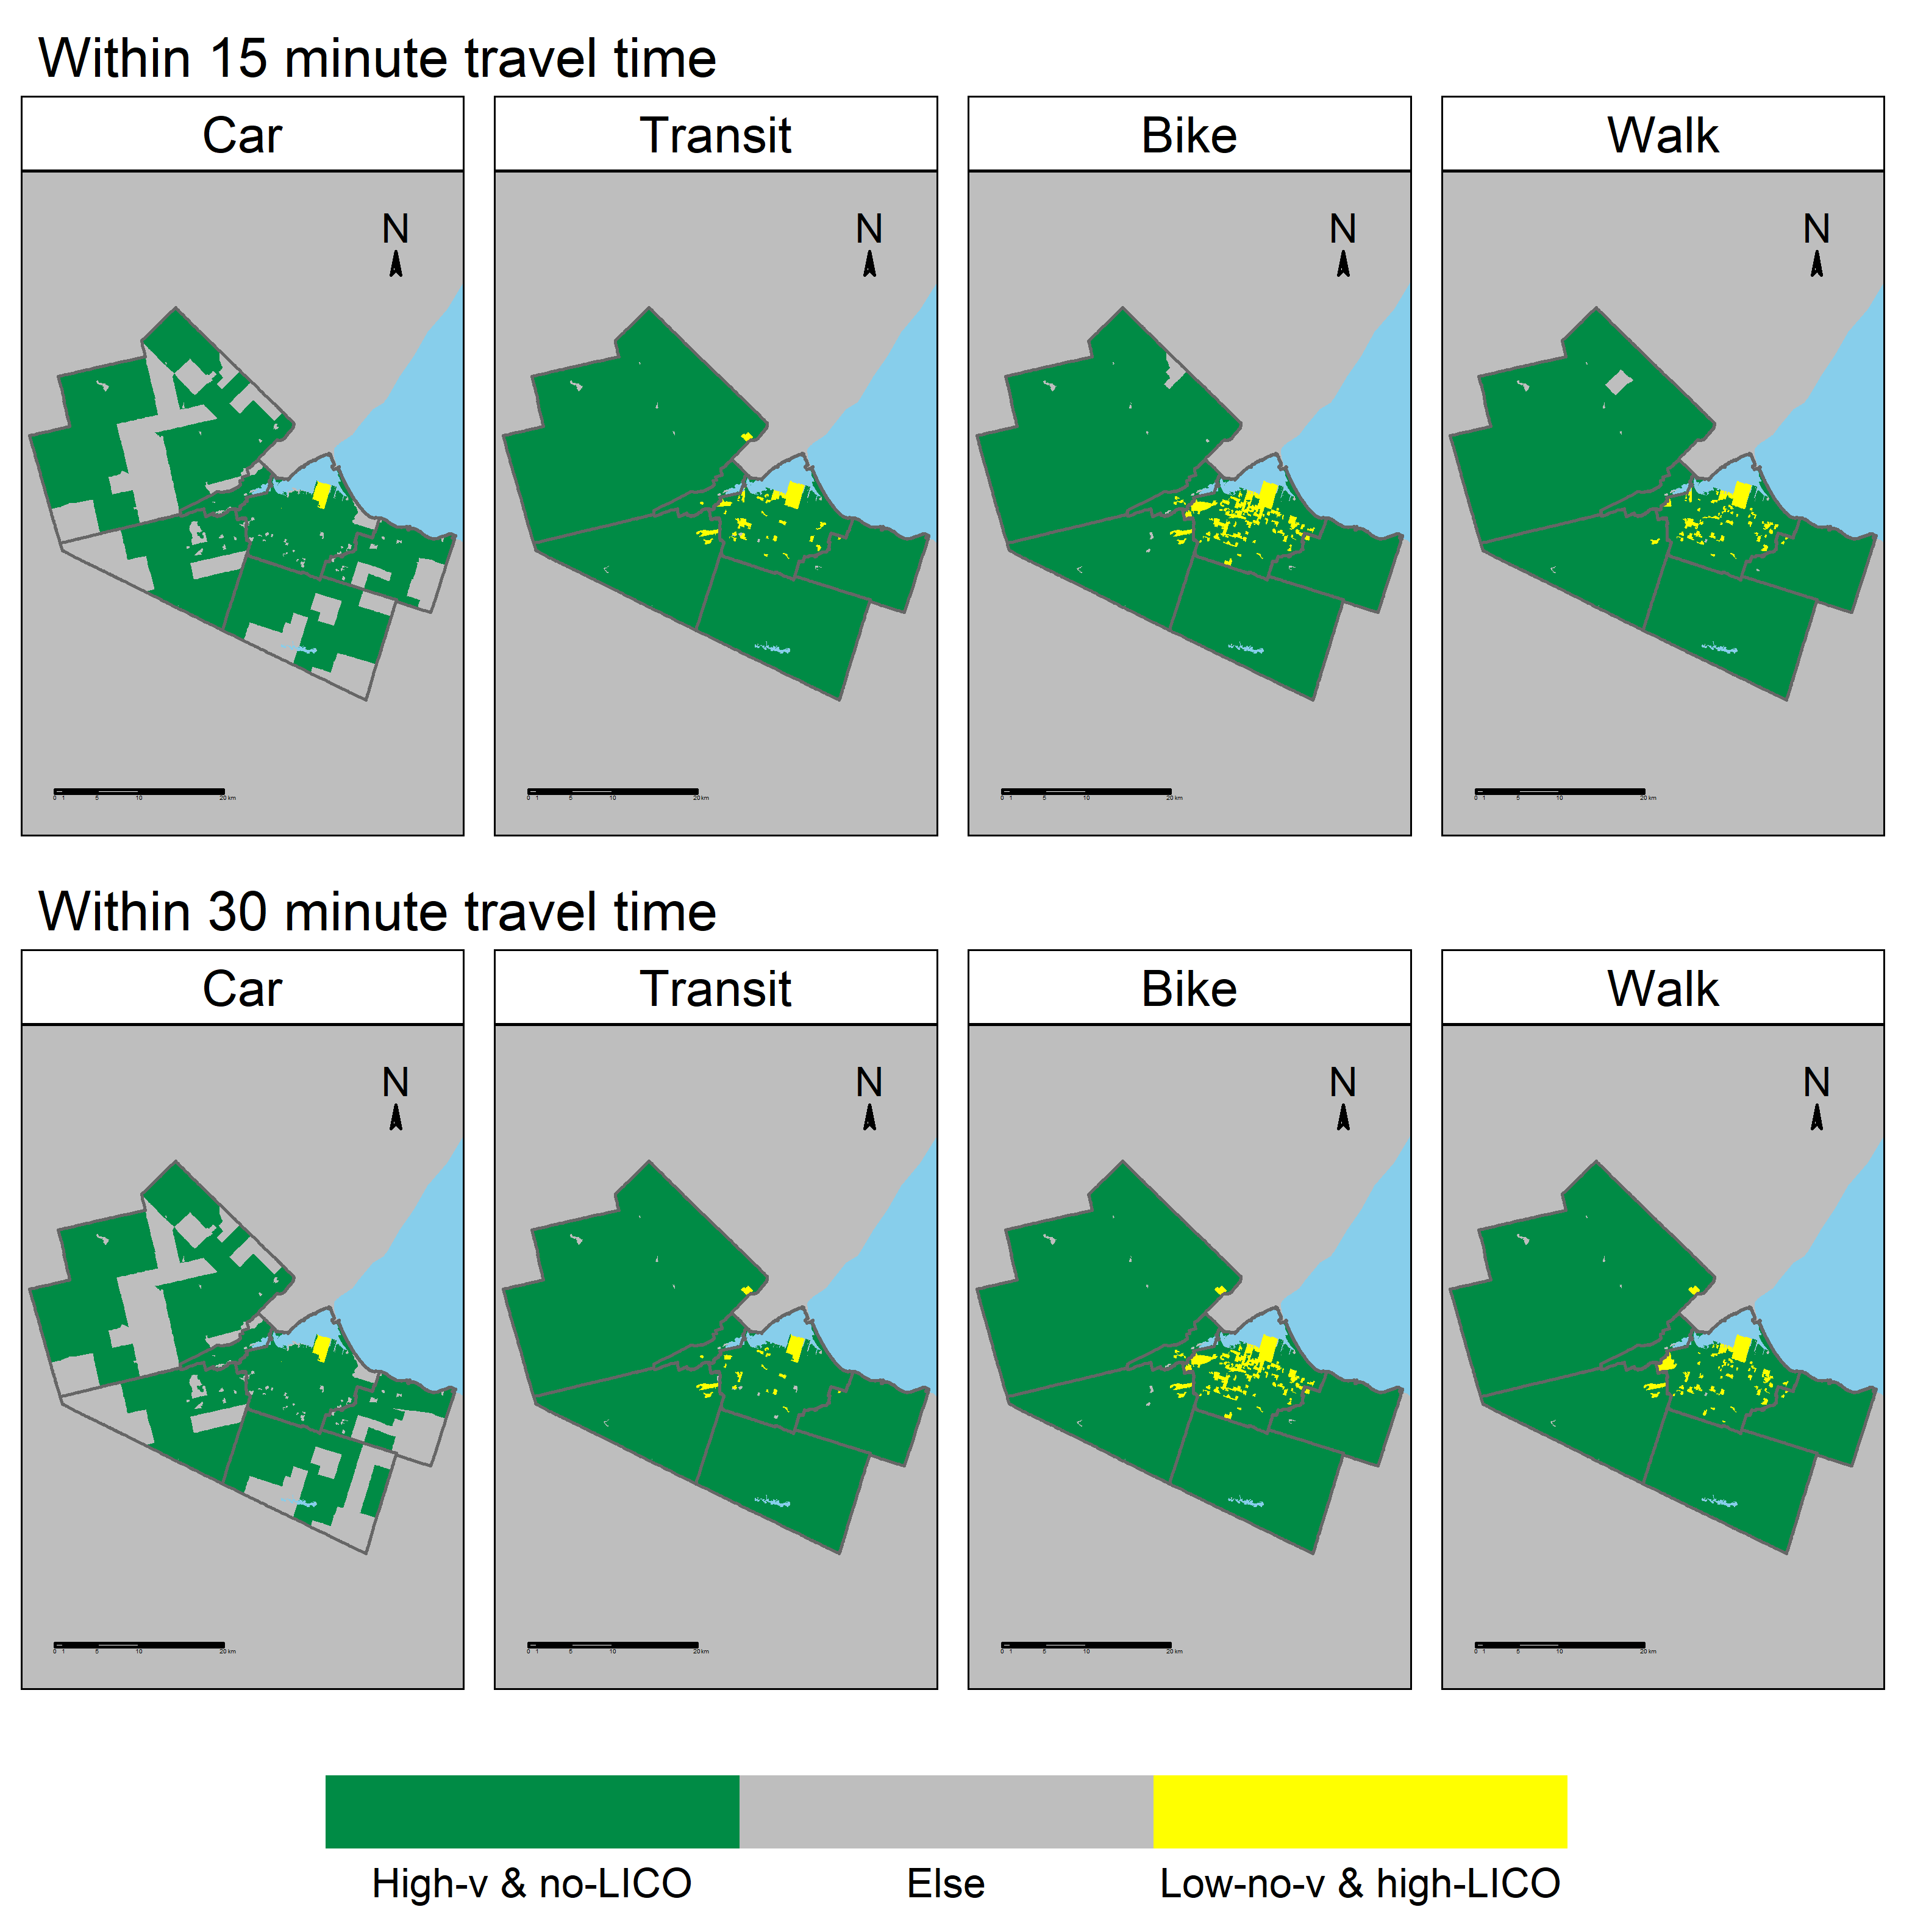
\includegraphics[width=6.25in,height=\textheight]{figures/Fig8-plot_Savail_smallv_LICO_measures.png}

}

\caption{\label{fig-Fig8}The spatial availability per mode-using-capita
measure versus high-income cut-off . The number of care destinations
that can be reached per mode-using-capita, per DA, within 15 mins (top)
and 30 mins (bottom). Basemap shapefiles are retrieved from the 2021
Canadian census \citep{governmentofcanadaCensusPopulation2023}, the Open
Data Hamilton Portal \citep{opendatahamiltonCityBoundary2023} and the
USGS \citep{greatlakesUSGS2010}.}

\end{figure}

Notice the green DAs for the car-driving population and presence of
yellow DAs for non-car modes within Hamilton-Central:
Figure~\ref{fig-Fig8} reinforces findings from Figure~\ref{fig-Fig6}.
Even in Hamilton-Central where there is high proportion of LICO-AT
prevalence, car-mode using populations who reside in green DAs are still
offered high levels of spatial availability. However, car ownership is
not always possible for low-income households and the lack of ownership
acts as a barrier to accessing economic and economic-support
opportunities for low-income households \citep{morrisDoesLackingCar2020}
when alternative modes are insufficient
\citep{kleinTransitionsOutCar2023}. For this reason, populations below
the LICO-AT may rely on non-car modes, and the introduction of policies
that increase access to care-destinations could be considered. The
majority of yellow DAs are within the centre of Hamilton-Central,
specifically for cycle- and walking populations. Policies that increase
the number of available care-destinations within Hamilton-Central,
improve conditions that decrease LICO-AT prevalence, as well as policies
that make car-modes less spatial availability advantaged (i.e.,
encourage modal shift and decrease travel time) could be further
investigated through the lens of mobility of care.

\hypertarget{discussion-and-conclusions}{%
\section{Discussion and conclusions}\label{discussion-and-conclusions}}

This paper is the first to conduct an exploratory feminist accessibility
analysis of care destinations -- one that counters the current
literature's emphasis on employment-related travel, a travel more
significant for men, and especially wealthy and educated men
\citep{lawWomenTransportNew1999, hansonGenderMobilityNew2010}. Its aim
is to challenge current planning paradigms by explicitly focusing on
care, vital and life-sustaining activities that are undervalued, and to
provide a tangible example of how one could gender-mainstream
accessibility analyses. In doing so, it contributes to the emergent
mobility of care literature, a body of what that has, to date, focused
on quantifying this under-represented type of travel
\citep{gomezvaroAccountingCareEveryday2023, murillomunarCaregiversMoveGender2023, ravensbergenExploratoryAnalysisMobility2022, sanchezdemadariagaMobilityCareIntroducing2013, sanchezdemadariagaMeasuringMobilitiesCare2019, shumanCanMobilityCare2023}
and has provided rich and nuanced qualitative accounts of lived
experiences completing mobility of care
\citep{orjuelaReconsideringMobilityCare2023, ravensbergenVelomobilitiesCareLowcycling2020, sersliRidingAloneTogether2020}.

This paper also contributes to accessibility research by implementing
both an unconstrained (cumulative opportunities) and constrained
(spatial availability) multimodal accessibility measure. The
unconstrained measure demonstrates the potential interaction with care
destinations that each mode offers from each DA within a 15- and 30-
minute travel time thresholds. The constrained measure incorporates the
assumed proportion of mode-using population and mode-specific travel
time to demonstrate the potential interaction with destinations that
each DA has available to a mode-using population. The distinction
between the constrained and unconstrained measures are clarified, namely
that potential interaction may be over-inflated, especially for the
lower range non-car modes, when considering unconstrained access over
spatial availability. Unconstrained access may demonstrate over-inflated
promise for active transport modes. The consideration of both
unconstrained and constrained access can encourage a shift in
perspective. Motorists are generally estimated high unconstrained access
to many care destinations as well as exceptionally high spatial
availability. Those who use alternative modes, have low unconstrained
access and, in certain DAs, and even lower level of availability. This
is as a result of car-using populations being allocated a
disproportionate number of total care destinations. Spatial Availability
is a way of conceptualising accessibility as a city-wide total and each
calculated value is a proportion so it can be easily placed relative to
all others in the city. However, it relies on assumptions on who is
``demanding'' the destinations, and how those assumptions are made are a
subject of ongoing discussion in how accessibility considers competition
\citep{merlinDoesCompetitionMatter2017, kelobonyeMeasuringAccessibilitySpatial2020}.

Further, this study contributes to the literature on sustainable travel
behaviour. Results indicate that care is most easily accessed in
Hamilton by car, an unsurprising result given its car-oriented design.
Previous research has found that mobility of care are more frequently
completed by car or by foot than by transit or by bicycle
\citep{ravensbergenExploratoryAnalysisMobility2022}. It is possible that
the car's ability to provide higher access to care destinations, as
observed in this study, shapes this tendency to complete care trips by
car. Car use may also be more frequent for care trips because these
trips tend to involve carrying things (e.g., groceries) or people (e.g.,
children). Indeed, past qualitative work has found that many prefer
travelling by car for this type of trip due to convenience and increased
safety
\citep{maciejewskaHaveChildrenThus2019, carverParentalChauffeursWhat2013}.
Then again, care trips tend to be shorter than other trips
\citep{ravensbergenExploratoryAnalysisMobility2022}, making them ideal
for more sustainable travel modes, such as active modes (walking,
cycling) and public transport. The low access to care by foot identified
in this study is discouraging, given both people's tendency to use this
mode for care trips \citep{ravensbergenExploratoryAnalysisMobility2022},
and the benefits of walking as a travel mode, both for individuals,
cities, and the environment. Somewhat unexpectedly, access to care was
found to be low by transit and by foot and relatively high by bicycle.
Given that low income women, in particular, seem to be transit reliant
for care trips \citep{ravensbergenExploratoryAnalysisMobility2022}, this
result highlights both a potential bias against care trips by transit
and the equity implications of that bias. Though past work has found
that many barriers exist for cycling for care
\citep{ravensbergenVelomobilitiesCareLowcycling2020, ravensbergenFeministGeographiesCycling2019, sersliRidingAloneTogether2020},
the results of this study highlight the great potential of the bicycle
for easily accessing care.

The preliminary nature of this research also comes with its limitations
as a result of data availability. The accessibility results are not
calibrated to reflect observed mobility-to-care travel behaviour due to
data unavailability nor are they formulated to express any normative
accessibility goals. Instead, they present a preliminary exploration of
how the mobility of care concept could be operationalised within
accessibility analysis.

First, the travel time estimations assume free-flow network conditions:
while impacting estimated travel times, estimated congested conditions
may not have a drastic impact on spatial accessibility calculations
\citep{yiannakouliasEstimatingEffectTurn2013}, especially for cycling
and walking modes. Second, the use of a binary travel time cut-off
instead of a more complex travel impedance function can have a
significant impact on accessibility results. To add reliability, two
literature-informed travel cost thresholds (15-minutes and 30-minutes)
were selected, but results' interpretation are hampered by the binary
function selection: some zonal populations could \emph{still} value
destinations beyond a 30-minute travel time, and some populations may
not see a destination 5 minutes and 15 minutes away as necessarily equal
in travel impedance. Third, the geometric centroids of DAs (origins) and
destinations (all care destinations) were used as inputs for travel time
calculations. DAs are created for the purpose of the census: they vary
in area and centroids may not necessarily align with where that
population may begin their journey to care destinations. Fourth, the
quality, importance and specific willingness to travel to types of care
destinations for mode-using populations within a zone was not considered
as data is unavailable city-wide. As such, this study assumes each
destination is 1 opportunity and re-weights each of the five care
categories to be conceptually equal. Fifth, the mode choice for care
destinations trips is unknown and hampers interpretation of spatial
availability. It is assumed in the study to be equal to the work-commute
mode selection, but this is may not be necessarily the case.

Future work could look to address these limitations as well as compare
access to care results to conventional access to work landscapes. This
comparison could highlight the bias in planning towards jobs as well as
substantiate equity critiques.

\hypertarget{references}{%
\section*{References}\label{references}}
\addcontentsline{toc}{section}{References}

\hypertarget{appendix}{%
\section{Appendix}\label{appendix}}


  \bibliography{bibliography.bib}


\end{document}
